%-----------------------------------------------------------------------------------------
% This template has designed by Mohamad Khaleqi
% You're very welcome to edit and use this template
% 2015-02-26
% Swansea University
%----------------------------------------------------------------------------------------

\documentclass[a4paper,12pt]{article}
\usepackage[utf8]{inputenc}
\usepackage[toc,page]{appendix}

\usepackage{lastpage} % Required to determine the last page for 
\usepackage{graphicx} % Required to insert images
\graphicspath{ {Figs/} }
\usepackage{comment} % Comment
\usepackage[utf8]{inputenc} 
\usepackage{url} % URL in Footnote  
\usepackage{cite} % BibLatex
\usepackage{listings} % hard code
\usepackage[document]{ragged2e} % Justify
\usepackage{wrapfig} % add picture wraped by text
\usepackage{arydshln} % add hash line for tables
\usepackage{booktabs} % new tables
%\usepackage[colorlinks,linkcolor=black]{hyperref}
\usepackage[colorlinks=false, linktocpage=false]{hyperref}
%{colorlinks=false, linktocpage=true}{hyperref}
\hypersetup{hidelinks}
\usepackage[fleqn]{amsmath}
\usepackage{mathtools}
\usepackage{pdflscape}
\usepackage{xcolor}
% \newcommand\mytodo[1]{\textcolor{red}{#1}}
\usepackage{lipsum}

\usepackage{tcolorbox} % colour box
\usepackage{float}
\usepackage{courier}
\usepackage{todonotes}
\usepackage{hyperref}
\usepackage{glossaries}

\makeglossaries

\usepackage[nottoc]{tocbibind} % add list of figure and tables and put them in content 

\usepackage{geometry}

% Margins
\topmargin=-0.45in
\evensidemargin=0in
\oddsidemargin=0in
\textwidth=6.5in
\textheight=9.0in
\headsep=0.25in 




\linespread{1.3} % Line spacing

%----------------------------------------------------------------------------------------
%	TITLE SECTION
%----------------------------------------------------------------------------------------

%----------------------------------------------------------------------------------------
%	TITLE SECTION
%----------------------------------------------------------------------------------------
\newcommand{\horrule}[1]{\rule{\linewidth}{#1}} % Create horizontal rule command with 1 argument of height
\title{
\begin{Huge}\textbf{INTERACTIVE VISUALISATION OF SHAKESPEARE'S OTHELLO} \end{Huge} \\% The assignment title
\vspace{70px}

\includegraphics[width = 65mm]{Figs/SwanseaUniversity}\\[8ex]
\begin{large} \textsc{\textbf{Xiaoxiao Liu}} \end{large} \\ % Your university, school and/or department name(s)
\begin{large} \textsc{\textbf{889170@swansea.ac.uk}} \end{large} \\ % Your university, school and/or department name(s)
\vspace{10px}
\normalfont \normalsize 
\begin{normalsize}Department of Computer Science \end{normalsize}\\  % Your university, school and/or department name(s)
\begin{normalsize} Swansea University \end{normalsize} \\ % Your university, school and/or department name(s)
\vspace{60px}
This dissertation is submitted for the degree of\\
\textit{Master}
\vspace{20px}
}
\author{} % Your name
\date{} % Today's date or a custom date


%------------------------------------------------------------------------------------
% Document begin
%------------------------------------------------------------------------------------
\begin{document}
\pagenumbering{gobble} %stop page number
%------------------------------------------------------------------------------------
% Page Title
%------------------------------------------------------------------------------------
\begin{titlepage}

\maketitle
\vfill
\center \date{\normalsize December 2017} % Today's date or a custom date
\end{titlepage}
% -----------------------------------------------------------------------------------

\pagenumbering{Roman} 
\justify

% ******************************* Thesis Declaration ***************************
\null\vspace{\fill}
\renewcommand{\abstractname}{\large }
\begin{abstract}
%\vspace{2cm}

\section*{Declaration}

This work has not previously been accepted in substance for any degree and is not being concurrently submitted in candidature for any degree.

December 15, 2016

Signed:

\section*{Statement 1}

This dissertation is the result of my own independent work/investigation, except where otherwise stated. Other sources are acknowledged by giving explicit references. A bibliography is appended.

December 15, 2016

Signed:

\section*{Statement 2}

I hereby give consent for my dissertation, if accepted, to be available for photocopying and for inter-library loan, and for the title and summary to be made available to outside organisations.

December 15, 2016

Signed:


\vspace{1cm}



\end{abstract}

\vspace{\fill}
% ************************** Thesis Acknowledgements **************************
\null\vspace{\fill}
\renewcommand{\abstractname}{\large Acknowledgements}
\begin{abstract}
\vspace{2cm}

And I would like to acknowledge ...
\end{abstract}
\vspace{\fill}

% ************************** Thesis Abstract *****************************
\null\vspace{\fill}
\begin{abstract}
\vspace{2cm}
William Shakespeare was one of the greatest writers the world has ever seen. His works have been translated and retranslated many times into many languages. Studying the variations of these translations is important to understand the evolutions for translation, culture, as well as history. A group of researchers in the College of Art and Humanities at Swansea University has a collection of different German translations of Shakespeare's play, \emph{Othello}. They attempt to study the variations of words between different translations, and to find unique words in certain translations. This project aims at creating an interactive visualization system of text data by providing a parallel view to compare varieties of text between translation versions. In addition to this, a software is designed to enable users to interact with the visualization. The data processed in this project contains 15 German translations of \emph{Othello} and a base text in English, collected by Dr. Cheesman from College of Arts and Humanities at Swansea University. Our goal is to provide visualization solutions that assist them to identify and analyse such words and translations. 




\end{abstract}
\vspace{\fill}


%------------------------------------------------------------------------------------
% Table of content
%------------------------------------------------------------------------------------
\tableofcontents
\pagebreak
\listoffigures
\pagebreak
\listoftables
\justify
%------------------------------------------------------------------------------------
% Document begin
%------------------------------------------------------------------------------------
\clearpage
\pagenumbering{arabic}
%-----------------------------------------------------------------------------------------


\section{Introduction and Motivation}
%-----------------------------------------------------------------------------------------

Data sets have risen dramatically over the past few years, and these data sets have become increasingly complicated to analyse. How to deal with large amounts of data has become a challenge in certain fields\cite{Larameea}. According to \cite{Ward2015}, when receiving large volumes of information, people tend to use sight as the main sense to understand it. Data visualization, as a mechanism  using graphics to represent data \cite{Ward2015}, provides a good solution for exploring huge sets of complicated data.

As stated by \cite{Williams1995}, data visualization is defined as "the visual representation of a domain space using graphics, images, animated sequences, and sound augmentation to present the data, structure, and dynamic behaviour of large, complex data sets that represent systems, events, processes, objects and concepts"\cite{Williams1995}. By applying techniques of data visualization, more information can be explored.

Text data emerges in large quantities every day in newspapers, blogs, and social media. Hence, extracting information from text data is becoming highly needed. In some certain study areas, studying the relationship between words, sentences and texts’ structure may help researchers to understand important information hiding in the text. For example, in an archaeological laboratory, analysing the text they found from a historic site may help them understand the dates of files, antecedent events, or the host of the grave, even without knowing the meaning of the ancient language. Similarly in the archaeological industry, techniques in text data analysis is fundamental and significant in translation study. Many institutes rely on knowledge of text data analysis to explore the variation of language in history, style of authors, as well as the social status of people in a particular period. 

The ways to analyse and present text data have become a popular topic as the volume of the text data is often huge and complicated in format, genre, and morphology. For instance, languages inherited from different roots may lead to different expressions when translating from one to another. Authors of different eras or regions may use different words to express the same things. The same contents may appear in different styles of expressions according to the purpose of the texts. Also, to deal with these problems, text data can be analysed and represented from lexical, syntactic and semantic perspectives \cite{Ward2015}, so that the unstructured text can be converted to structured data. Calculating frequency and weights of words can help to explore the information of content. There have been plentiful tools to visualize the structure of text data, such as Word Clouds, Word Tree, Tex Arc, etc. And for different research purpose, text data are often analysed separately in a single document and a collection of documents. One such collection of documents is \emph{Othello}.

\emph{Othello}, as one of the greatest tragedies of Shakespeare's plays, has been translated more than 60 times in German  \cite{Geng2011}.The College of Arts and Humanities at Swansea University has a collection of 55 different German translations of \emph{Othello}. The time span of these translations range from 1766 to 2010. And there are also different genres such as poems and prose, as well as plays. Applying data visualization techniques to help represent these text data will contribute to new research in the study of Shakespeare's work, and explorations into visualization. More concretely, the aims of this project are as follows:

\begin{itemize}
	\item \textbf{}To develop an interactive visualization system that enable the researchers in the College of Art and Humanities to explore detailed translation information of different versions.
	\item \textbf{} To design a software of textual data visualization to display more information by compare different versions of translations, such as time span, genre, interpretation.
	\item \textbf{} To explore potential solutions in textual data visualization for difficulties in translation comparison, such as parallel text and data filtering.
\end{itemize}

Using textual data visualization as an aid to explore the text data of \emph{Othello}’s translations will  benefit for researchers to understand the changes, interactions, and impacts of these translation versions and cultures, time span, and styles \cite{Alrehiely2014}. Based on the work of \cite{Geng2015}, \cite{Alrehiely2014}, and \cite{Tom2012},we attempt to develop an interactive visualization system aimed to allow our users to view, compare, and analyse tokens in each version. The visualization tool will be designed to assist in viewing the variation of tokens in different translation versions, and in comparing the varieties of tokens after applying different methods to process the text data. Apart from the essential information about each version, such as the author and data of publication, there are three unique fields the data provides: the frequency of tokens, weight of tokens, and results from lemmatization for tokens.

The outcomes of the visualization system should be helpful in understanding the variation of word morphologies, varieties of text styles, and the complex features of the German language. It also facilitates improved comprehension of literature dynamics, the differences between languages, and the perception of translating cultures. Moreover, this project will provide a visualization tool for books, articles, newspapers, etc., to represent large sets of text data.  

The German Shakespeare text data in this project, several special problems are caused by antiquated language, and poetic orthography. The former means that some words used in the 18th or 19th century may not be in the lexis of training corpora, if these are based on 20th/21st century sources. And by using the poetic orthography, take “verloren" (meaning: lost) for example, the word is normally written as “verloren", though can also be spelled verlor'n, or verlorn in some places in Shakespeare texts (the word normally has 3 syllables, pronounced VER-LOR-RUN, but the writer wants it to be spoken as 2 syllables, VER-LORN). This kind of situation happens a lot. Yet there are no effective algorithms to recognise these forms. To find a solution to these problems, some methods from Natural Language Processing may be applied, such as lemmatization.

Choosing this project for my dissertation was on account of my interest in the field of data visualization and language analysis. The background of programming and language study will further my comprehension of data analysis and processing. Developing a project such as Translation Visualisation is becoming a significant topic for language studying and text data processing.

Following \cite{Laramee2011}, the rest of this thesis is structured as follows: Section 1 to section 4 are modified versions of work previously presented by the author in \cite{Liu}. Section 2 details the background research, along with the literature review, introduction to existing systems, and data characteristics. Section 3 details the specifications of the project, which includes the features specification of software and technology choices. Section 4 presents the approach of the project, time arrangement and potential risks. Section 5 provides an overview of project design. Section 6 describes how the project is implemented. In section 7, we provide the performance and feedback from a domain expert as an evaluation. Section 8 draws a conclusion of this project, and section 9 discusses potential further work. 


%-----------------------------------------------------------------------------------------
\clearpage
\section{Background Research}
%-----------------------------------------------------------------------------------------

In this section, a literature review is first introduced to present the most relevant works to this project. In the second part, previous systems in a similar project are introduced. The third part provides a detailed analysis of the data characteristics.

\subsection{Literature Review}

This section defines principles and techniques for data preprocessing and text data visualisation.

Text Visualisation Browser \cite{Kucher2014} is an online tool which provides the most comprehensive summary of published text visualisation \cite{Cao2016}. According to the Text Visualisation Browser, from 1976 to 2017, there exist 400 published text visualisation papers in total, in which 396 publications are aimed to analyze text alignment. By searching ’Word’, there shows 20 publications, and ’Translation’ gets 16 results. Whereas when typing ’Frequency’ and ’Weighting’, each keyword gets one results. Also, keywords such as ’Machine learning, ’Data Mining’, 'Natural Language Processing' got no result found. 

The results indicate that in the text visualisation domain, most researchers focus on presenting alignment of texts. There is some focus on topics such as ’word analysis’ and ’translation’, which is similar to this project. However, applying more specific techniques such as ’Natural Language Processing’ haven’t been applied in text visualisation widely.


\paragraph{Interactive Exploration of Versions across Multiple Documents}

\paragraph[]{}In the work of \emph{Interactive Exploration of Versions across Multiple Documents}, \cite{Jong2008} provide an interactive visualisation tool,
MultiVersioner, to address the issues of comparing several versions of texts. The MultiVersioner enables users to search for items such as words, phrases and lines, along with the analysis of the frequency patterns of these items. In addition, methods such as colour-coded highlighting and overview are also rendered in this tool. Figure \ref{fig:multiVersioner} shows an example of an overview for many versions and documents in this software. In the overview, terms are denoted by blocks. If user mouses over a single block, a tooltip with the relevant sentence will be popped up.

\begin{figure}[H]
	\centering    
	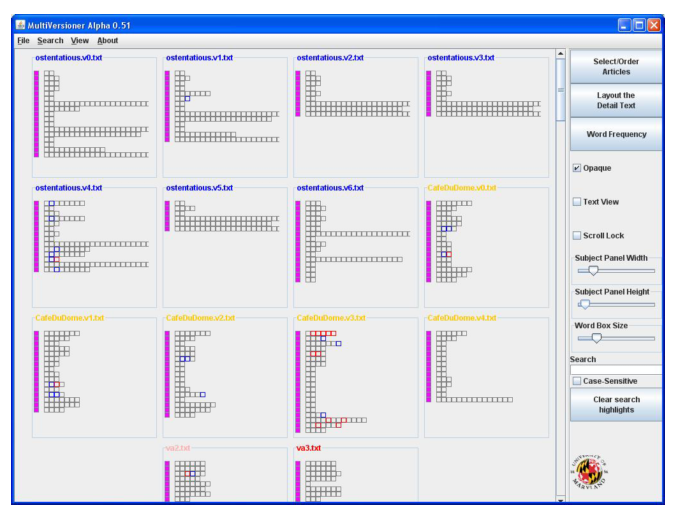
\includegraphics[width=\textwidth]{Figs/MultiVersioner}\\[1ex]
	\caption{An overview of many versions and documents in MultiVersioner (\cite{Jong2008}).}
	\label{fig:multiVersioner}
\end{figure} 

The work of MultiVersioner allows users to compare multiple documents. Meanwhile, it provides a helpful feature to search for entities such as words and lines. Moreover, it can be served as a tool to analyse the frequency patterns of the words. However, there are only limited features provided by this software. Some helpful functions such as alignments between versions, or version toggling need to be explored.

\paragraph{Interactive Visual Alignment of Medieval Text Versions}
\paragraph[]{}

\cite{Stefan2017} discussed novel methods to compare text versions in the work \emph{Interactive Visual Alignment of Medieval Text Versions}. They provide a visual analytics system which enables computationally aligned complex textual differences such as orally inflected text. 

The data they deal with is a group of medieval poetries with complex text forms. Their works include three basic visualisations:

\begin{itemize}
	\item \textbf{A visualisation of text alignment} This is a visualisation in which highly unstable text versions are identified and aligned. This feature is accomplished applying a parameter-driven approach. Moreover, a visual analytic process is rendered which accepts tweaking parameters for iterative improvement of the alignment.
	\item \textbf{Multi-level alignment visualisation} In this view, various visualisations are presented which enables users to analyse texts alignments on different hierarchy levels.
	\item \textbf{Meso Reading} This is a visualisation to interpret texts in parallel. Similarly, the connections are demonstrated among text versions. This is considered as a novel feature which provides an intermediate perspective to display complex variance in texts.
	
Figure \ref{fig:mesoReading} is an interpretation of this project. The screenshot in \cite{Stefan2017} displays different views of the distant reading, the meso reading, the close reading, and full-line matches. In part one, distant reading results of high similarity on words are displayed in the form of parallel lines. In addition, diagonal lines represent several repetitions. In part two, meso reading results are shown in the verse line ’Qui me dist que li ange sont’.  In part three, a close reading feature is explored to show false positive alignment while part four are matches for numerous full-line text.
	
	\begin{figure}[H]
		\centering    
		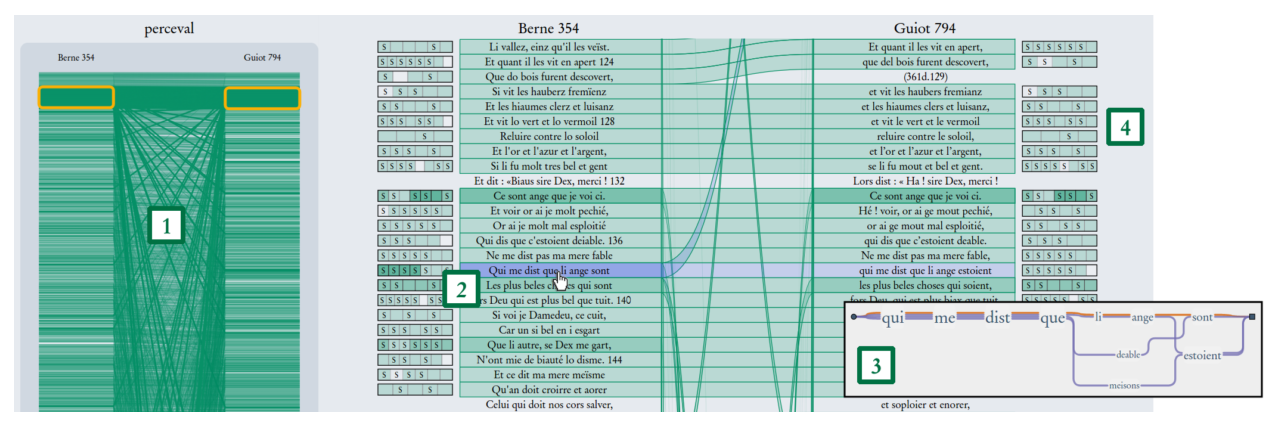
\includegraphics[scale=0.5]{Figs/Meso-Reading}\\[1ex]
		\caption{ (1) distant reading (2) meso reading (3) close reading (4) full-line matches (\cite{Stefan2017}).}
		\label{fig:mesoReading}
	\end{figure} 
	
	
\end{itemize}

However, this tool is more suitable for French context, which limited the rage of data text can be processed applying methods in this work.

\paragraph{Visualizations Translation Variation of Shakespeare's \emph{Othello}: A Survey of Text Visualisation and Analysis Tools}
\paragraph[]{} In their work \emph{Visualizations Translation Variation of Shakespeare's \emph{Othello}: A Survey of Text Visualisation and Analysis Tools}, \cite{Geng2011} developed a visualisation system which can be used to view and analyse variations between translation text and based text. The data of this project is a collection of German translations of Shakespeare’s \emph{Othello}. In this project, several techniques are applied to get an interactive visualisation system. These techniques include parallel coordinate, Treemap, and DOI-tree. The tools which they developed provides features that enable users to brush words so that these words can be displayed in a parallel tag cloud. Figure \ref{fig:tagCloud} is a screen shot which illustrates the outcome of applying the TagCrowd feature into one of Othello translation version. In this view, the stop words are identified and removed manually from the original text.

\begin{figure}[H]
	\centering    
	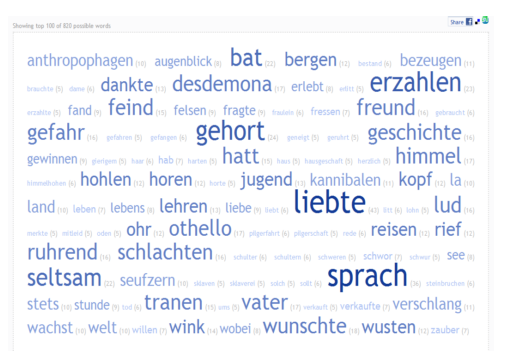
\includegraphics[scale=1]{Figs/Tagcloud}\\[1ex]
	\caption{The TagCrow (\cite{TagCrowd}) visualisation of a passage from \emph{Othello}.}
	\label{fig:tagCloud}
\end{figure} 

\paragraph{ShakerVis: Visual Analysis of Segment Variation of German Translations of Shakespeare’s \emph{Othello}}
\paragraph[]{} ShakerVis \cite{Geng2015} is a special visualisation tool which is designed to provide an interactive visualisation system to display version variations. In this system, \cite{Geng2015} applies following visualisation techniques:

\begin{itemize}
	\item \textbf{Parallel Coordinate View} provides outcomes by using the Eddy value. The description of Eddy value can be seen in Previous System chapter.
	\item \textbf{Scatter Plot View} presents an average similarity value for each translation across multiple segments.
	\item \textbf{Term-document Frequency Heat Map} renders a way to analyse differences between pairs of versions in details, including a measurement of character-string similarities.
	
\end{itemize}

\subsection{Previous Systems}

The Version Variation Visualization (VVV) project was introduced by Dr Tom Cheesman from the Modern Language Centre at Swansea University. It aims to create interactive data visualisation system to build cross-cultural exploration networks. The VVV project focus on developing digital tools which can help to compare and analyze different versions of translation \cite{Cheesman2012}. So far, the tools developed in the project are Ebla, Prism and ShakerVis.  Ebla, served as the corpus, is a software to stock the text data and detailed information about them.  Prism provides the interface for separating texts into segments and processing the segments as alignment. Based on the idea of this two software, ShakerVis provides an interactive interface for visualizing the information of the translation versions \cite{Geng2015}.

There are three types of data visualisation in this project: Time-Map, Alignment Maps, Parallel view and Eddy and Viv view. 

\paragraph{Time-Map}
\paragraph[]{} 

Figure \ref{fig:timeMap} supplies a screen shot of Time Map, which shows the location of the authors and the year of translation for the versions published.  From this view, we can guess that some particular places such as Berlin and Dresden in which more authors were born this places published more translaitons versions. This can be deemed as that these two cities are popular places with large scale of city.

\begin{figure}[H] 
	\centering    
	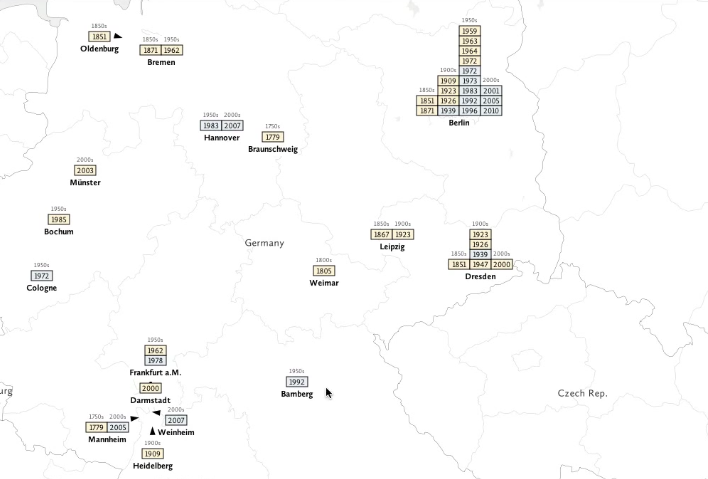
\includegraphics[scale=0.7]{Figs/Time-Map}\\[1ex]
	\caption{A demo screen shot for Time-Map (\cite{Cheesman2012}).}
	\label{fig:timeMap}
\end{figure} 

\paragraph{Alignment Map}
\paragraph[]{}

Figure \ref{fig:alignmentMap} exhibits a parallel visualisation which provides an alignment from the segments in the base texts to the translation versions. The yellow parts highlighted the whole segment selected while the blue line serves as the alignments. By comparing these texts, one can tell the general differences between the base text and translations. For example, if one segment of certain translation is longer than that of the base text, it is possible that a particular expression in German is appeared. 

\begin{figure}[H] 
	\centering    
	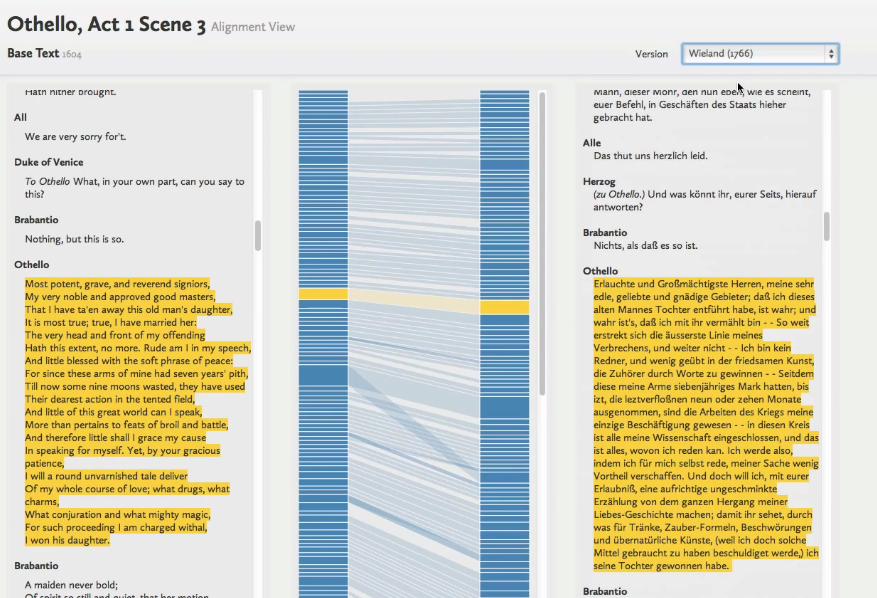
\includegraphics[scale=0.7]{Figs/Alignment-Map}\\[1ex]
	\caption{A screen shot of the demo of Alignment Maps (\cite{Cheesman2012}).}
	\label{fig:alignmentMap}
\end{figure} 

\paragraph{Parallel View}
\paragraph[]{}

Parallel View provides an explicit view between the base text and selected version. Figure \ref{fig:parallelView} shows a straightforward view of base text and selected translations.  In this visualisation, segments are more explicit to find.

\begin{figure}[H] 
	\centering    
	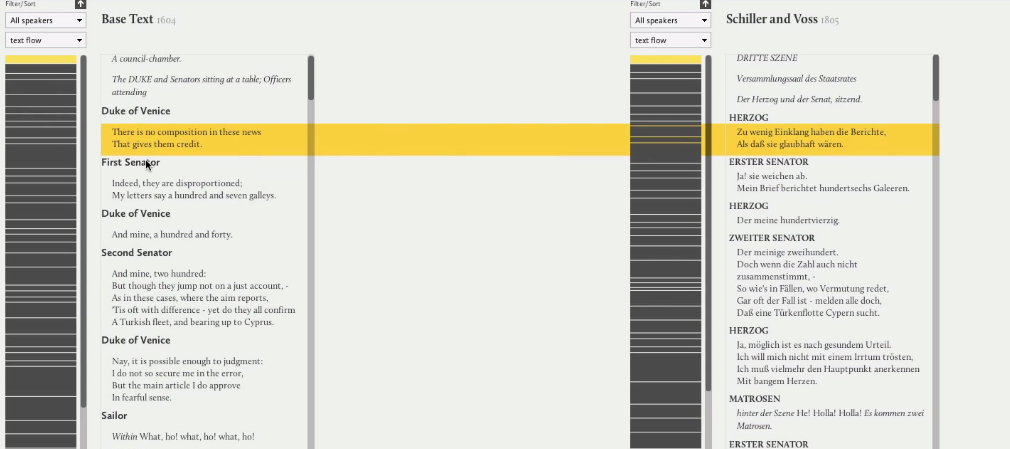
\includegraphics[scale=0.6]{Figs/Parallel-View}\\[1ex]
	\caption{A screen shot for the demo of Parallel View (\cite{Cheesman2012}).}
	\label{fig:parallelView}
\end{figure} 

\paragraph{Eddy and Viv View}
\paragraph[]{}

Eddy and Vis view enable researchers to understand more details   of the vocabulary. Figure \ref{fig:eddyVivView} demonstrates Eddy and Viv view, which provides more information of the translation comparison. From the sort bar, we can tell that there are four types can be visualized. Eddy value shows the variation of words used in the segment. Relatively, Viv value provides the changes or rivalries for some segments in translation.  If we choose version name, segment length or reference date as the order of sorting, there will be other information on translation variations. 

\begin{figure}[H] 
	\centering    
	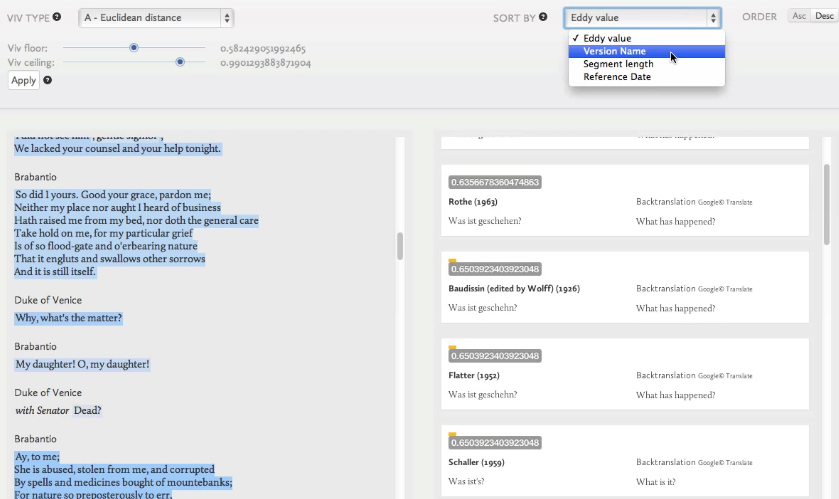
\includegraphics[scale=0.6]{Figs/Eddy-Viv-View}\\[1ex]
	\caption{A screen shot of Eddy and Vis view (\cite{Cheesman2012}).}
	\label{fig:eddyVivView}
\end{figure} 




%-----------------------------------------------------------------------------------------
\clearpage
\section{Project Specification}
%-----------------------------------------------------------------------------------------
This part is the specification of the project which includes the features specification and technology choices to the software. The user features the system will also be stated. The project specification discussed in the initial document is modified and updated here as a section of the final dissertation.

\subsection{Data Characteristics}

Data is a major part of all visualisation, which along with user experience play an important role as "driving factor" with respect to the choice and attributes of the visualization method \cite{Laramee}. In this chapter, the data relevant to this project is analysed, including the type, size, format, and characteristics of data. Also, a description of data preprocessing will be discussed. 

The data sets used in this project come from a collection of 57 different German translations of \emph{Othello}, which is contributed by Dr. Tom Cheesman, from College of Arts and Humanities at Swansea University, working on a project in \cite{Tom2012}. To develop analytic tools and probe the translations in this corpus, the team digitalized 32 translation versions, with the formats being normalized, texts being segmented, speech by speech and line by line. The content of these 32 texts corresponds to Act1, Scene 3 of the English version of \emph{Othello} (1604) play as the base text. Based on this corpus, we are given 15 text files of German translation versions by Dr. Tom Cheesman for this project. And together with the base text in English, these 16 text sets are read and processed when implementing the project.All these files are encoded as UTF-8 when converting from .docx format to .txt format. The number of words in each document are different according to the genres of text data (327 words at maximum, and 214 words at minimum). Figure \ref{fig:dataExample} is a screen shot of the text data used in the project. All data has been segmented and cleaned
\begin{figure}[H]
	\centering    
	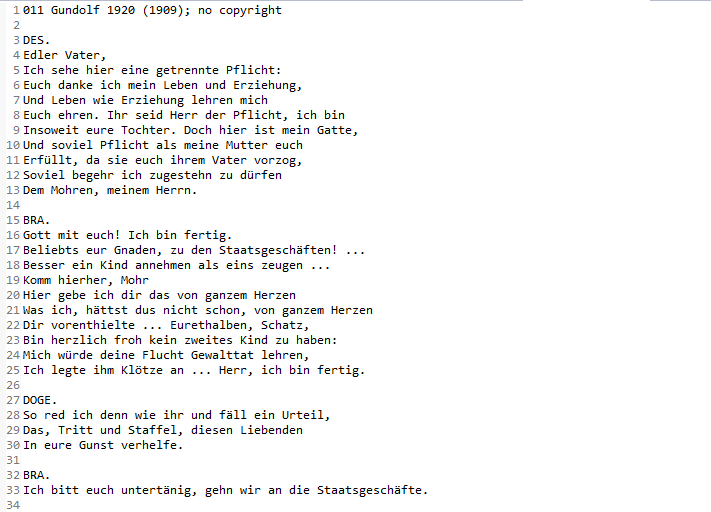
\includegraphics[scale=0.8]{Figs/Data-example}\\[1ex]
	\caption{A screenshot of text data used in this project.}
	\label{fig:dataExample}
\end{figure}
The text file is commonly used to store plain texts data. It is a simple text file format which can be worked with many programming languages, including Java. Choosing .txt file as the data set is owing to following reasons:

\begin{itemize}
	\item \textbf{} The aim of this project focuses on word processing, which requires computers to read text literally, without applying complicated data processing techniques.
	\item \textbf{} Since the text data sets in the corpus are stored in .docx format which is difficult to read directly from Java, it is easier and safer to convert the .docx format into .txt format.
	\item \textbf{} There exist methods in Java.io, a Java API, used to read .txt data directly from files.
	\item \textbf{} Apart from the basic and simple information (publication year and author) of each version, there is no need to obtain more information from the text. Additionally, because the data set in each version is not large, the computer can calculate the essential features of the data, in a short time, every time the program is ran. 
\end{itemize}


\subsection{Feature Specification}
This project is aimed at developing an interactive visualisation for a group of different text documents. The result of this visualisation should assist users in identifying and exploring the variations between these translation versions. The software has following features:
\begin{itemize}
	\item \textbf{} Provide an interactive visualisation system.
	\item \textbf{} Develop a user interface serves as a tool for users to select options.
	\item \textbf{} Read and store data from .txt files.
	\item \textbf{} Provide a parallel visualisation for comparing terms in different translation versions.
	\item \textbf{} Generate concordance view with frequency bars
	\item \textbf{} Add author and publish year as the title of each concordance.
	\item \textbf{} Provide a visualisation with scroll bars.
	\item \textbf{} Connect same words in each concordance applying coloured edge.
	\item \textbf{} Provide user option for scaling the visualisation.
	\item \textbf{} Scale the size of window.
	\item \textbf{} Generate a colour mapping view, and the colour represents the frequency of words.
	\item \textbf{} Render a user option for turning translations on and off.
	\item \textbf{} Create an English-German word translation index.
	\item \textbf{} Add user option: highlight the bar and connection when clicking single bar.
	\item \textbf{} Provide user option: highlight bars with same frequency when clicking a block in colour legend.
	\item \textbf{} Generate a Lemma and Frequency visualisation.
	\item \textbf{} Generate a Tf-Idf Visualisation.
	\item \textbf{} Generate a Lemma and Tf-Idf  Visualisation.
\end{itemize}
\subsection{Technology Choices}
According to the project specification and required features presented previously, the demonstration of technology choices is made in the following chapter.
\subsubsection{Programming language}
For the implementation of the software in this project, Java programming language is selected to develop the software. Java has known that it is an object-oriented language and class-based \cite{Gosling2014}. It is also simple enough to understand fast. With years of upgrading and improvement, it has been growing into a mature programming language. This also means using Java to develop software will have fewer mistakes and bugs when programming. There are also active communities on the internet, in which lots of people share useful ideas and resources of Java. In addition, due to the limitation of background which is not Computer Science, the author is more familiar with Java programming language.  

\subsubsection{Java Library}

\paragraph{Java Swing Library}
\paragraph[]{} The Java Swing Library is the tool we used in this project to generate GUI of the software. This is a free, cross-platform resource which is appropriate for using Java in implementing this project.

\paragraph{Stanford NLP Library}
\paragraph[]{} The Stanford NLP Library is attempted during we generate the lemma for English version text \cite{StanfordNLP}. This is a free and open source for Natural Language Processing. However, because this library has not provided German lemmatisation function, we adopted other solutions in this project.

\subsubsection{Other Techniques}

\paragraph{TreeTagger}
\paragraph[]{}TreeTagger, developed by Helmut Schmid at the Institute for Computational Linguistics of the University of Stuttgart \cite{TreeTagger}, is a tool for annotating text data and lemma information. It has been used to tag many languages including German.

\paragraph{Github}
\paragraph[]{} For source code backup requirement, the Github is adopted. The main software we used most is the GitKraken (See Figure \ref{fig:gitKraken}), which provides an interactive user interface to commit project. As a version control tool, the Github helps in organizing the development process of our software and in keeping an updated version of the software.

\begin{figure}[H]
	\centering    
	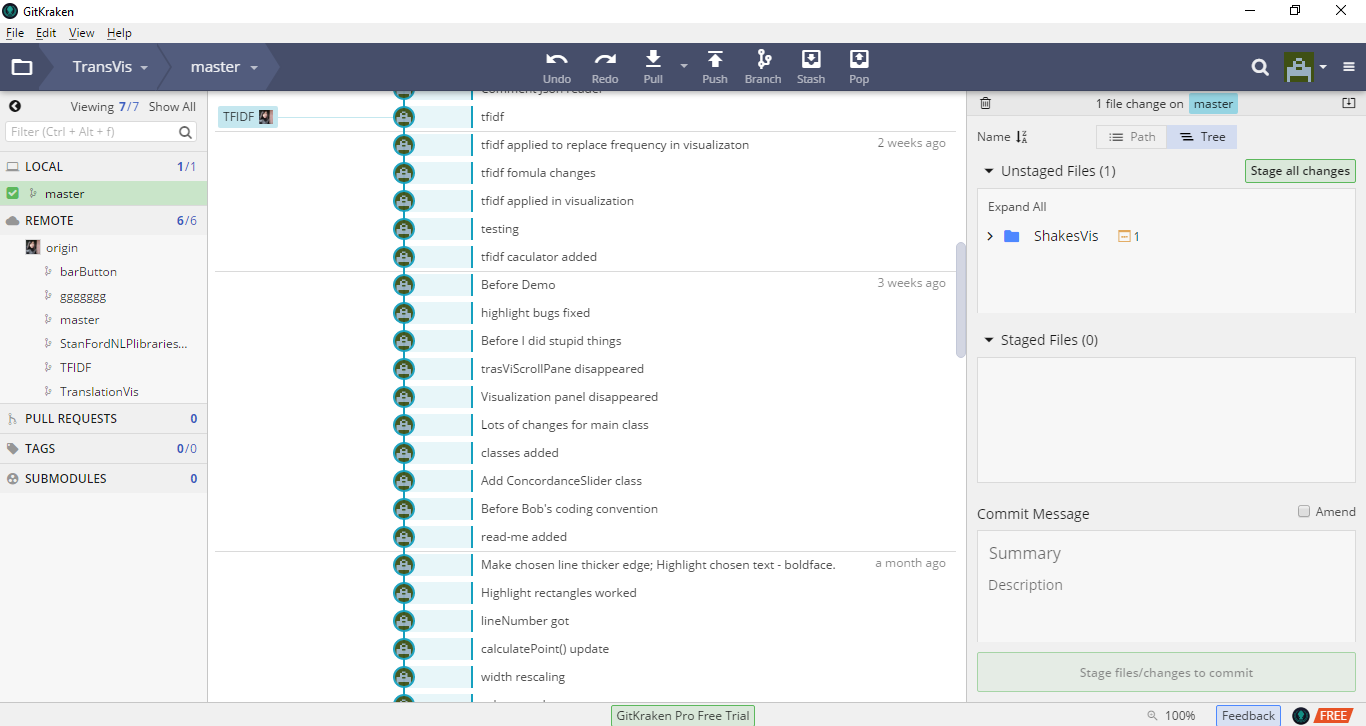
\includegraphics[scale=0.4]{Figs/GitKraken}\\[1ex]
	\caption{A screenshot for the user interface of GitKraken.}
	\label{fig:gitKraken}
\end{figure}

\paragraph{Dropbox}
\paragraph[]{} The Dropbox is another backup software which can be used to store data. We adopt this software to store our source data in the case that equipment is broken, or the website of Github is collapsed.
\textit{}
\paragraph{Eclipse and Visual Studio Code}
\paragraph[]{} Eclipse and Visual Studio Code are tools we used in this project for Java programming. The Eclipse is the main tool to program in Java, while the Visual Studio Code serves as a backup software in the case that Eclipse is collapsed. 

\paragraph{Notepad++}
\paragraph[]{}The Notepad++ is a free and useful tool for source code editing. It also supports editing files in many kinds of format. In this project, we adopt Notepad++ to encode data during Data Processing phase.

%-----------------------------------------------------------------------------------------
\clearpage
\section{Project Plan and Time Management}
%-----------------------------------------------------------------------------------------

 

\subsection{Development Approach}

Traditionally, =Waterfall Model is used as the guiding methodology for many projects. It uses linear flow to show the progress of the project and allow people to understand easily the further steps after completing the previous step. It is suitable for sequential design, which means it may be impossible for developers to back to steps if they found some problems at last. 
The progress of the Waterfall Model is, according to\cite{Adenowo2013}, include 5 phases: Requirement analysis, design, implementation, testing, and operation and maintenance.(See Figure \ref{waterfall})

\begin{figure}[H]
	\centering	
	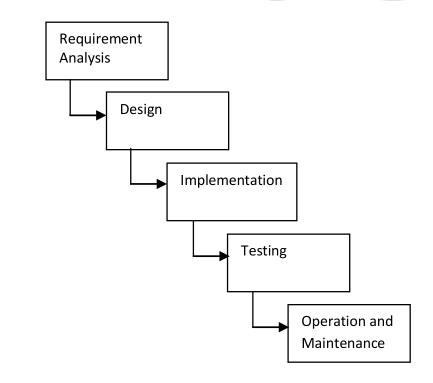
\includegraphics[width=6cm, height=6cm]{Figs/Waterfall-Model}\\[1ex]
	\caption{The 5 phases of Waterfall Model ( \cite{Adenowo2013})}
	\label{fig:waterfall}
\end{figure}

However, when projects run out of time, testing phase will be cut, which may lead to poor quality of the outcomes. In addition, the operation is in the last step, developers may be unaware of where they’ve gone and what they’ve done, it is invisible for developers to know the progress. Last but not least, it is impossible for developers to change until the last phase.

\begin{figure}[H]
	\centering	
	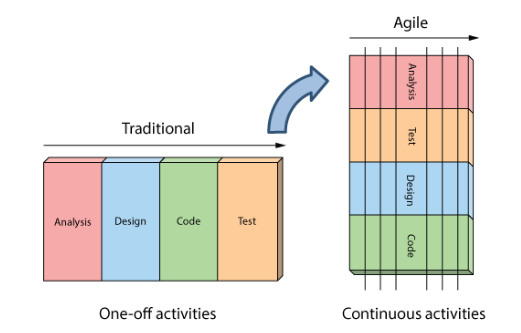
\includegraphics[width=6cm, height=6cm]{Figs/Waterfull-Agile}\\[1ex]
	\caption{Comparison between Waterfall methodology and Agile methodology (\cite{Agile vs Waterfall})}
	\label{fig:waterfallAgile}
\end{figure}

Unlike with the Waterfall methodology which separates the whole project into several phases and implement it step by step, the Agile methodology separates the project into several tasks and every task is implemented in several phases. By doing this, it is changeable for developers when they find mistakes. And hence the quality and visibility issues of Waterfall methodology are solved. Hence, we adopt Agile as our guiding methodology when implementing this project.

\subsection{Project Timetable}

This section indicates time management for the project. These project separates into 5 phases \cite{Laramee} as follow:

\begin{itemize}
	\item \textbf{1. }Requirements Specification; 
	Data Preprocessing; 
	Project Presentation;
	Exploring existing tools; 
	Project Specification; 
	 complicated data processing techniques.
	\item \textbf{2. }Software Design;
	Candidate Classes and Responsibilities;
	Candidate Hierarchy;
	Collaboration and Subsystems;
	\item \textbf{3. }Implementation;
	Software Development;
	GUI;
	\item \textbf{4. }Debugging and Testing;
	\item \textbf{5. }Documentation;
\end{itemize}

Figure \label{gantterChart} indicates the Gantt of the project timeline. This project initiated from 17th February, and the final deadline is 30th September. In every phase, there are several tasks to be done. Most of the tasks in phase one has been done, except data preprocessing which needs more time to process more text data. The second phase is expected to finish before July. So more can be used in the implementation phase. Software implementation is supposed to spend the most time, which will be executed according to the designs done by previous work. After the implementation, simple GUI framework will be done. From the middle of August, the project is expected to start debugging and testing phase. Finally, a report and Doxygen will be done in September. 

\begin{figure}[H]
	\centering	
	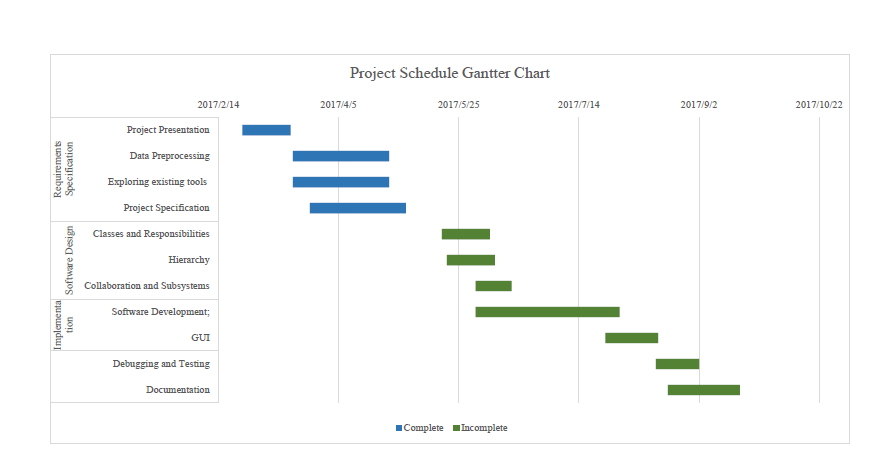
\includegraphics[width=16cm, height=14cm]{Figs/Gantter-Chart}\\[1ex]
	\caption{Gantt chart for project timeline }
	\label{fig:gantterChart}
\end{figure}


\subsection{Risk Analysis}

This part is about the potential risks which may happen when doing this project.

Figure \label{riskAnalysis} mapping the analysis of these risks:\.
The first risk is that the author may lack of the knowledge when carrying out the project. The probability is medium as the limited time author has been studying the computer science. The impact has been considered as high because the project will progress slowly and face obstacles without support of essential knowledge. So, the regular meeting with the supervisor is important to consult the difficulties encountered during the process.   
The second risk is that the whole project may be finished after the deadline. The possibility is considered medium due to the possibility of other risks. Lack of essential knowledge, problems in programming, or lack of project management skills may lead to the delay. The author should apply for delaying submission if this will happen in advance. 
The third risk identified is personal illness of the author. It is a low possibility risk with medium impact for the project. To deal with this case, keeping a good healthy is important to author herself. In addition, there is welfare service department on campus and the author has the international student’s insurance. 
Equipment failure is identified as the fourth risk. It is classified as medium in terms of both possibility and impacts. Yet there are computer equipments on campus and the library open 24 hours so that the resources of university are available every day. 
Data loss is considered as the fifth risk. the possibility of this happening is low but will cause high impact to the project. To avoid this situation, using the application Github for regular backup is necessary. 
The last risk is lacking project management skills to implement the project. This is considered as medium possibility to happen with high impacts to the project. In this case, a strict plan following rules of Agile software development methodology is important.

\begin{figure}[H]
	\centering	
	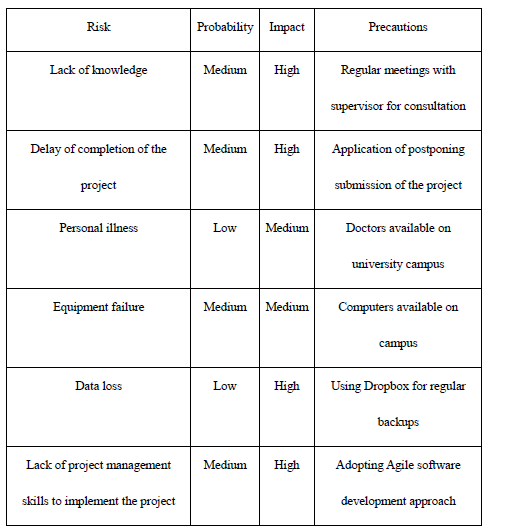
\includegraphics[width=15cm, height=18cm]{Figs/Risk-Analysis}\\[1ex]
	\caption{Risk Analysis Table }
	\label{fig:riskAnalysis}
\end{figure}


%-----------------------------------------------------------------------------------------
\clearpage
\section{Project Design}
%-----------------------------------------------------------------------------------------
 
 The design starts with a list of classes and their responsibili- ties. This is a very important starting point (the list of classes and descriptions). It forces the programmer to start thinking about implementation.
 After identifying a list of candidate classes and writing a short description of each of them, e.g., 3–4 sentences, the list is reviewed with the project supervisor before proceeding onwards with the description of relationships between them.

\subsection{Data Reading}


\subsection{Visualization Generation}

\subsection{GUI}

%-----------------------------------------------------------------------------------------
\clearpage
\section{Implementation}
%-----------------------------------------------------------------------------------------
In this section we describe how the project is implemented in detail. The subsystems executed are data reading, visualization rendering and the user options. Screen captures of the GUI are added to illustrate further information.

\subsection{Data Processing}

The main concept of data processing is to read text data from .txt files, calculate values need, and store them into Java Arraylist. At this stage, the greatest challenge is to keep the data being accessible and can be changed, as  the new data may be written over the old due to events in other class. Hence, after the original data is read and stored, it is retrieved and modified through  mutator methods \cite{Bob's coding convention}. In addtion to the flexibility, another difficulty at this stage is generating values for each term and store them appropriately. As discussed in the Project Features section, the aim of the software we designed is to present information about terms and provide an concordance view for each version. In this project, we calculate and sort frequencies of terms; compute colour values; computed locations of strings; instantiate Rectangle objects to represent data; create arrays to store translations.

Java.io, which enables for system input and output through data streams \cite{javadoc java.io}, is used in this project. It serves as a data buffer and reader in this project. The FileReader class, which extends the InputStreamReader class, can be used to read character files which by default are assumed to be an appropriate size. Since the volume of data in each document is not large, we instantiate a FileReader (object) to access each text file. The other data reading class adopted is the BufferedReader class. It is used to read text data from a character-input stream, and buffer the data to provide efficient reading of strings, arrays and lines \cite{javadoc7}. Java.util is another package imported in the DataReader class. To store and access data, the ArrayList, Hashtable, and Map classes from this package are used. In addition, classes such as JsonObject, JsonReader, and JsonArray in Javax.json package are used to read data from a Json file.

The main class that is responsible for reading the original data file is the DataReader class. This class analyses .txt files and generates a list of Version objects to parse all information needed in the software. Each Version object stores information of the concordance. For a more detailed description of the Version class and Item class, please see the Design section.

\subsection{Generating Concordances}

Concordances are the most basic visualisation in this project. They are designed to display the information of terms, and to help in comparing the terms between different translation versions.As shown in the Figure \ref{fig:condorVis}, the concordance visualisation involves several parts:
\begin{figure}[h]
	\centering	
	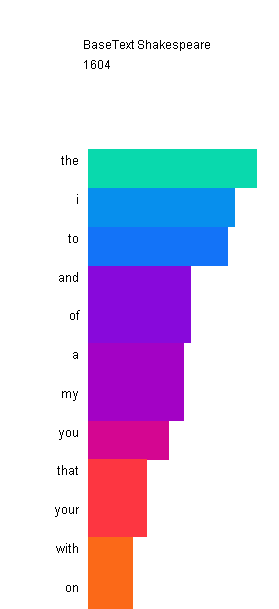
\includegraphics[width=9cm, height=15cm]{Figs/condordanceVis}\\[1ex]
	\caption{The Screen shot of one concordance in the visualisation}
	\label{fig:condorVis}
\end{figure} 

\begin{itemize}
	\item \textbf{String} is drawn to display the term, frequency, version author, publication year; 
	\item \textbf{Rectangle} is used to present the frequency. As the values are sorted in data processing phase, the width of rectangles are set according to these sorted values.
	\item \textbf{Colour} is used to present differences on frequency. Each colour represents a number of frequency, so there will be same colours in different terms.
\end{itemize}

The process in generating the concordance visualization goes through the following steps:
\begin{itemize}
	\item \textbf{} Obtain the string of each term from text source. This step is done in the DataReader class. Detailed illustration seeing Data Reading implementation section.
	\item \textbf{} Calculate the number of times, namely term frequency, of each term occurred in the text (See Data Reading implementation section).  	
	\item \textbf{} Calculate the rectangle width for each term using the frequency of term. The equation of the rectangle width calculating is show in Equation \eqref{rectWidth}:
	
	\begin{multline}\label{rectWidth}
	rectWidth=wordFrequency*unit*scaleValue
	\end{multline}
	
	Where unit is the width of each segment since the rectangle is composed of a number of segments. WordFrequency is the value deciding how many segments compose the rectangle, while scaleValue is the percentage value used to scale the rectangle, range from 10\% to 200\%.
	
	\item \textbf{}Calculate the location of the string and rectangle.The location, or point, is the start drawing point for the string and rectangle. It combined with two point value: point.X, and point.Y. The Equation \eqref{PointX}, \eqref{PointY} illustrate how we calculate these points in the software:
	
	\begin{multline}\label{PointX}
	point.x=versionNumber*versionDistance*scaleValue
	\end{multline}
	
	\begin{multline}\label{PointY}
	point.y= lineNumber*lineDistance*scaleValue
	\end{multline}
	
	Where versionNumber represents order number of the version. versionDistance performs the  distance between two neighbour versions. In addition, a scale value need to be multiplied so that the location of string and rectangle changes according to user preference.
	Similarly, the lineNumber is order number of the term while lineDistance represents the distance between two terms. 
	
	\item \textbf{}Calculate the value of colour. According to \cite{Jbum}, we use the equation as shown in Equation \eqref{Red}: 	
	\begin{multline}\label{Red}
	color = Math.sin(colorFrequency*wordFrequency + phase) * amplitude + center
	\end{multline}
	Where colorFrequency is a constant that controls how fast the wave oscillates. The wordFrequency is  variable used to display different colour according to word frequency. The phase is applied to change the alignment of the green or blue sine waves. The amplitude controls how high (or low) the wave goes. The center controls the center position of the wave.
	
	\item \textbf{}Paint the strings, blocks, and colours by invoking drawing methods in Graphic class. 
	
\end{itemize}

\subsection{Parallel View of Concordances}

Following the generation of concordance visualization, a parallel view of all concordances is created. As shown in Figure \ref{fig:parallelConcor}, all versions of concordances are represented on the panel. During this stage, lines will be drawn to connect same terms. The comparison stage is done in concordancePanel class. 

\begin{figure}[h]
	\centering	
	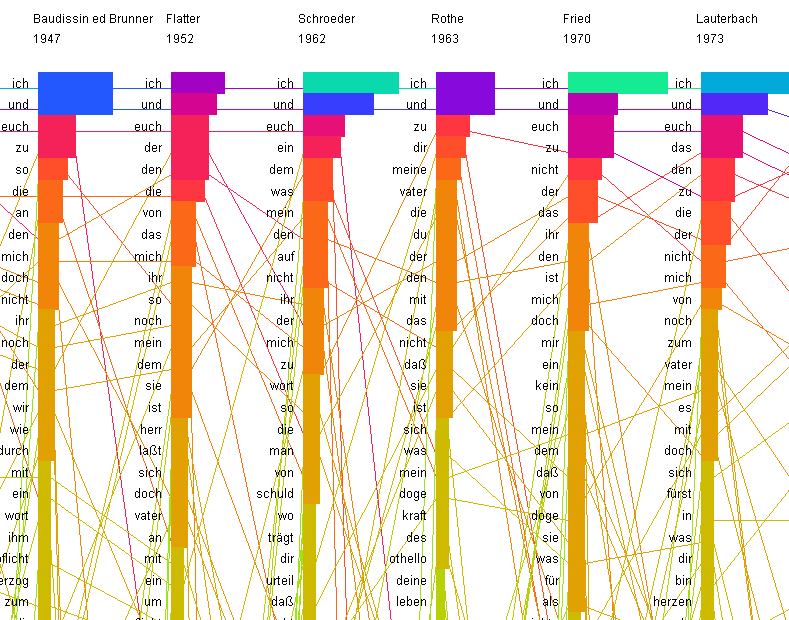
\includegraphics[width=13cm, height=8cm]{Figs/Parallel-Vis}\\[1ex]
	\caption{Parallel view of concordances}
	\label{fig:parallelConcor}
\end{figure} 


However, after this parallel visualization is being generated, an obvious problem appears: there is not enough space for all 16 concordances. So the solution is either to scale the panel, or to select several versions showing one time. We have done both, which are introduced in the following section. 

\subsection{Zooming}

Zooming in and out is a basic feature in the software which designed to provide two zooming options: one is for scaling the content of the visualisation, the other is for scaling the frame. In addition to these two scaling options, there are also scroll bars used to scroll the visualisation panel.

To implement these features, several steps as followed are gone through:
\begin{itemize}
	\item \textbf{} Generate the JSlider objects. This is carried out in the TranslationVisualization class. Figure \ref{fig:jSliders} displays the JSlider applied in the software.
	\begin{figure}[h]
		\centering	
		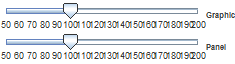
\includegraphics[width=9cm, height=3cm]{Figs/JSliders}\\[1ex]
		\caption{ Sliders applied to zoom in and out the graphic and panel}
		\label{fig:jSliders}
	\end{figure} 	
	\item \textbf{} Obtain scale values from JSlider object and pass them to DataReader class.
	\item \textbf{} Recalculated the data by invoking the calculating methods such as calculatePoint() and setRectWidth().
	\item \textbf{} Update the List<Version> object.
	\item \textbf{} Repaint graphics.
\end{itemize} 
 
During this process, the most difficult part is to recalculate all values of graphics: points, widths and heights for rectangles, and the distances between versions. To overcome this dilemma, two solutions are attempted:
At the first phase, scale() method in Graphics2D class is invoked. By applying this method, computer will calculate and repaint all the graphics using scale parameters passed in. However, when the project prompting to the Term Selecting phase (See Interactive Selection of Terms section below), a problem of obtaining mouse clicking location appears. Hence, the second phase of scaling visualisation comes out.  

At the second phase, scale values attained from JSlider objects are passed to DataReader class and applied in relevant formulas to calculate variables such as points, widths and heights of rectangles. See Equation \eqref{rectWidth}, \eqref{PointX}, and \eqref{PointY}. As shown in \ref{fig:jSliders}, 100 is set as the initial value for the slider, so that the visualisation shown when the visualisation generated at the first time is scaled as 100\%. Figure \ref{fig:zoomIn} and Figure \ref{fig:zoomOut} show the zooming results for the visualisation.

	\begin{figure}[h]
	\centering	
	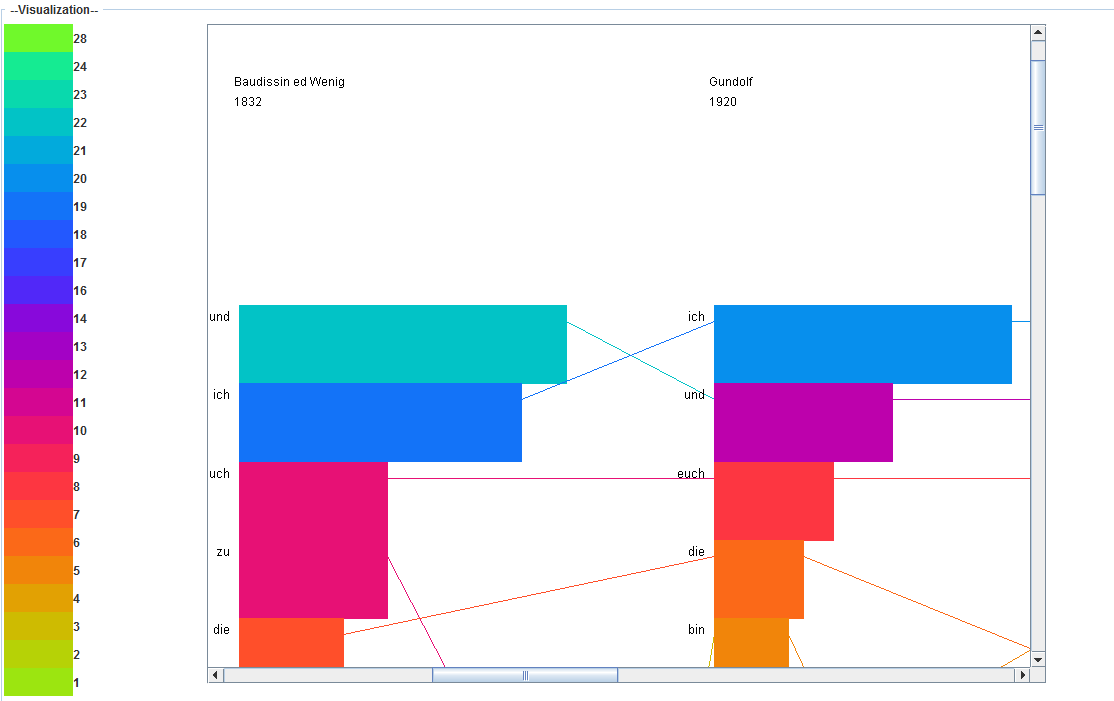
\includegraphics[width=9cm, height=3cm]{Figs/Zoom-In}\\[1ex]
	\caption{}
	\label{fig:zoomIn}
	\end{figure}

	\begin{figure}[h]
	\centering	
	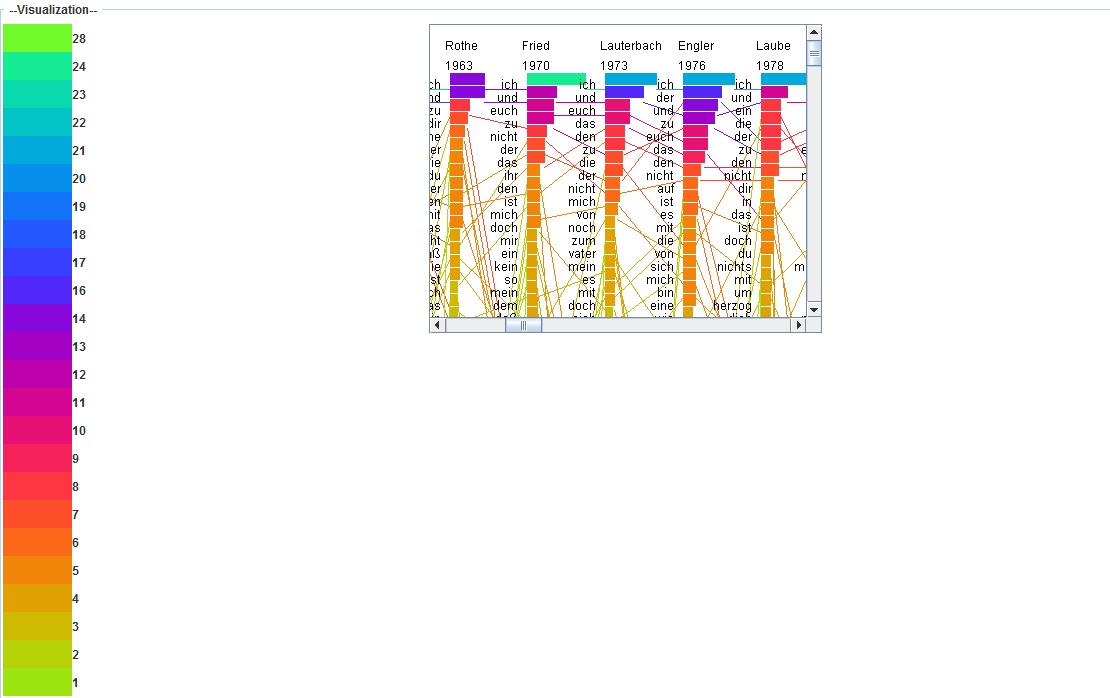
\includegraphics[width=9cm, height=3cm]{Figs/Zoom-Out}\\[1ex]
	\caption{}
	\label{fig:zoomOut}
	\end{figure}

\subsection{Text Labels On and Off}

When the scale values becoming smaller, the strings overlap. Hence a new desire appearing: hide strings on the visualisation. So that users can focus on the rectangles and colours only. 

To implement this feature, a JButton is generated on the panel firstly. Also, "Text On" is set as default label displayed on the button. Secondly, event listener is added to the button. When button is clicked, the label "Text On" on the button will be switched to "Text Off" label. In the meantime, a boolean value which set "true" as default will change to "false", then being given to ConcordancePanel class. In the third step, a boolean value preset when drawing strings of terms will be switched equals to the boolean value passed in. if it is "true", then draw the strings, if it is "false" then not invoke the drawString() method. At last, repaint the graphic. Figure \ref{fig:textOnOff} is a screen shot when we turn off the text.

\begin{figure}[h]
	\centering	
	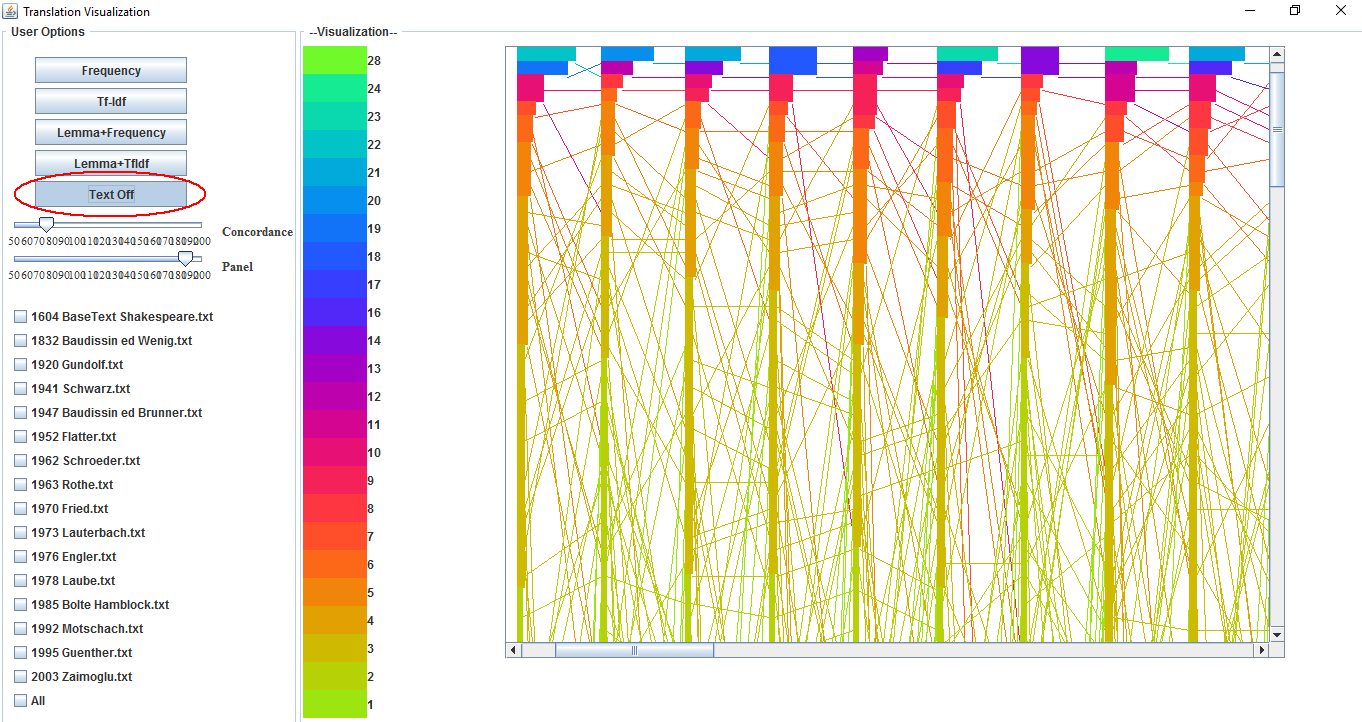
\includegraphics[width=18cm, height=12cm]{Figs/Text-On-Off}\\[1ex]
	\caption{}
	\label{fig:textOnOff}
\end{figure} 

\subsection{Adding, Subtracting, Selecting Items}

To render an user option feature for selecting several concordances displaying on the panel, a new class called VersionChoosenPanel is created. By interacting with this feature, not only can the user select which concordance to display in the visualization, but also the order of concordance displayed can be arranged. Figure
\ref{fig:versionChoosPanel} reveals the menu of version list can be selected. 
\begin{figure}[h]
	\centering	
	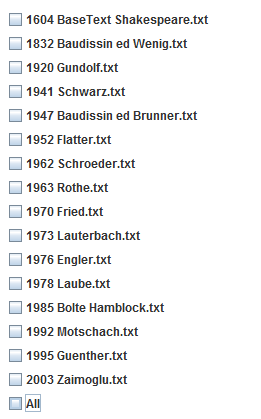
\includegraphics[width=6cm, height=10cm]{Figs/VersionChoosePanel}\\[1ex]
	\caption{The index of version selection}
	\label{fig:versionChoosPanel}
\end{figure} 

The generation of version selection feature goes through the following steps:
\begin{itemize}
	\item \textbf{} Generate a list of JCheckBox class to display the author name as the index. 
	\item \textbf{} Add event listener for each JCheckBox object. So that the action of selection can be generated as an Object class.
	\item \textbf{} Change the selecting status of the index. 
	\item \textbf{} Generate new list of Version objects according to the events passed from JCheckBox ActionListener. Every time the user select a name in the index, a new list of Version objects will be generated and passed to ConcordancePanel class. 
	\item \textbf{} Repaint the concordance visualisation. The ConcordancePanel will be repainted by invoking repaint() method.
	\item \textbf{} Add an option of "All" selection, which is responsible to display or hide all concordances as the original order.
\end{itemize}

Figure \ref{fig:versionChoosDemo}is a screen shot of selecting several versions of concordances to show on the visualisation. Further more, concordances are reordered on the visualisation, where the base text which supposed to be shown as the first version on the left, now being moved to the last one.

\begin{figure}[h]
	\centering	
	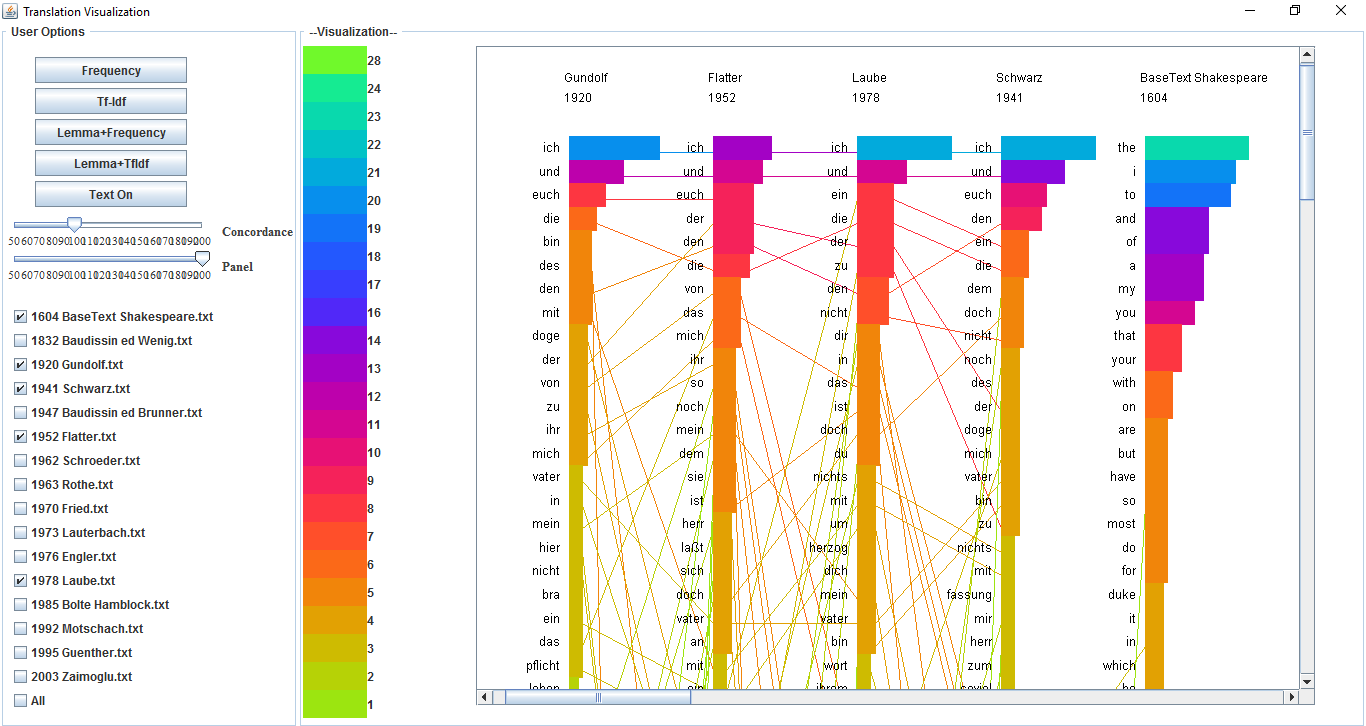
\includegraphics[width=18cm, height=10cm]{Figs/Version-Selecting-Demo}\\[1ex]
	\caption{The screen shot of version selecting feature}
	\label{fig:versionChoosDemo}
\end{figure} 

\subsection{Interaction and Selection of Terms}

On the ground that each concordance contains a large number of terms, highlight the term following users' options is desired. In order to provide an interactive features for terms, new feature are enable in the visualisation. Therefore a clear view of highlighting terms comes out. 

This features are achieved by put into effect following phases:
\begin{itemize}
	\item \textbf{} Obtain clicking point through getPoint() method in MouseEvent class.
	\item \textbf{} Calculate which item region the point belongs to. In this process, the regions of concordance and item are divided as illustrated in Figure \ref{fig:regionDivide}. As the value of each region can be achieved during data reading phase, the point passed from mouseClikcked() method can be used to identify which region the point belongs. Further more, the Item object of this block is singled out and returned.
	\begin{figure}[h]
		\centering	
		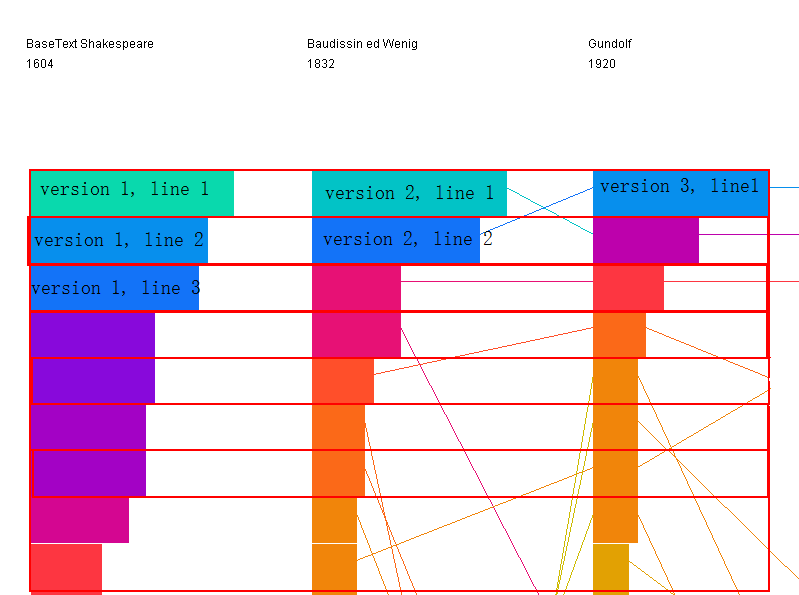
\includegraphics[width=6cm, height=10cm]{Figs/Region-Divide}\\[1ex]
		\caption{}
		\label{fig:regionDivide}
	\end{figure} 
	\item \textbf{} Identify the Item objects in other concordances sharing the same term. So that we get Item objects to be highlighted.
	\item \textbf{} Highlight the blocks of all singled out Item objects. In this step, lines are drawn to round the rectangles. 
	\item \textbf{} Make other blocks transparent. The transparency values of other rectangles are set as  semitransparent values by overwriting colour values of blocks.
	\item \textbf{} Overwritten the colour values of all lines to make sure lines connecting two highlighting items are highlighted as well, while other lines becoming semitransparent.
	\item \textbf{} Find out the translations of this term and highlight the blocks of them.	
\end{itemize}

As a result, by clicking one single rectangle in the panel, the rectangle is highlighted and rounded by line while the colour of other rectangles become transparent. In the mean time, lines connecting same terms become highlighted by setting other lines transparent. See Figure \ref{fig:highlightView}

\begin{figure}[h]
	\centering	
	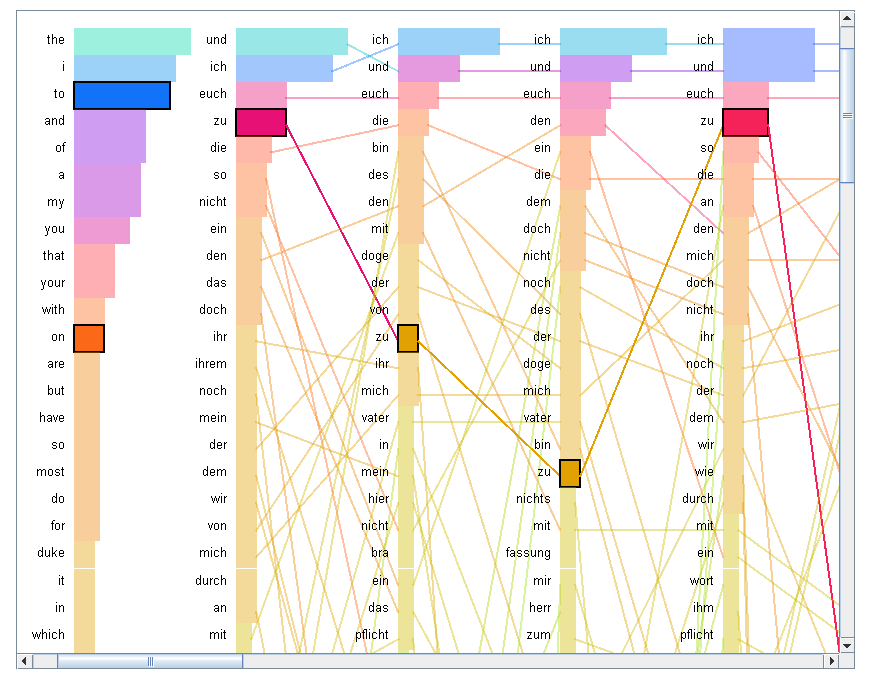
\includegraphics[width=16cm, height=9cm]{Figs/Highlight-Terms}\\[1ex]
	\caption{}
	\label{fig:highlightView}
\end{figure} 

\subsection{Colour Mapping}

Colour represents the occurrences of terms in each concordance. To demonstrate all colours in the visualisation, colour mapping is essential. In this project, we instantiate a ColorLegendPanel class to fulfill this feature. In addition, values of the frequency is displayed in the Colour Mapping view. Following is the process to implement this function: 
\begin{itemize}
	\item \textbf{} Achieve the colour value of each item from DataReader object. The detailed illustration of colour values can be retrieved in Data Reading chapter.
	\item \textbf{} Instantiate JLabel objects as the components representing colours.
	\item \textbf{} Add the JLabel objects to the panel.
	\item \textbf{} Display frequency values beside colour blocks.
\end{itemize}

The demo of Colour Mapping is shown in Figure \ref{fig:colourMapping}.
\begin{figure}[h]
	\centering	
	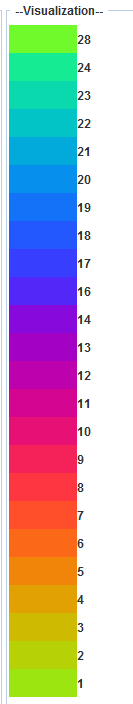
\includegraphics[width=4cm, height=15cm]{Figs/Color-Mapping}\\[1ex]
	\caption{}
	\label{fig:colourMapping}
\end{figure} 

\subsection{Interactive Color Legend}

Apart from displaying data, colour mapping can be served as interactive visualisation. In this project, we add an feature so that user can interact with the colour legend. If the user click a label of colour in the colour legend, all blocks of that colour in the concordance view will be highlighted. This function is performed by identifying all items possessing same frequency value. As illustrated in the Design chapter, an index of frequency values is generated in DataReader class. After data reading phase, we can access this list of frequency values through accessor method. By iterating all values in the list, the items are identified and returned to ConcordancePanel class. Then the list of Version objects are overwritten and the panel is repainted.

As a result, by clicking one colour block in colour legend, all items sharing same frequency, or colour, are highlighted using same methods of highlighting described in Interaction and Selection of Terms chapter. Figure \ref{fig:interactiveColourMapping} serves as a demo to illustrate this feature.
\begin{figure}[h]
	\centering	
	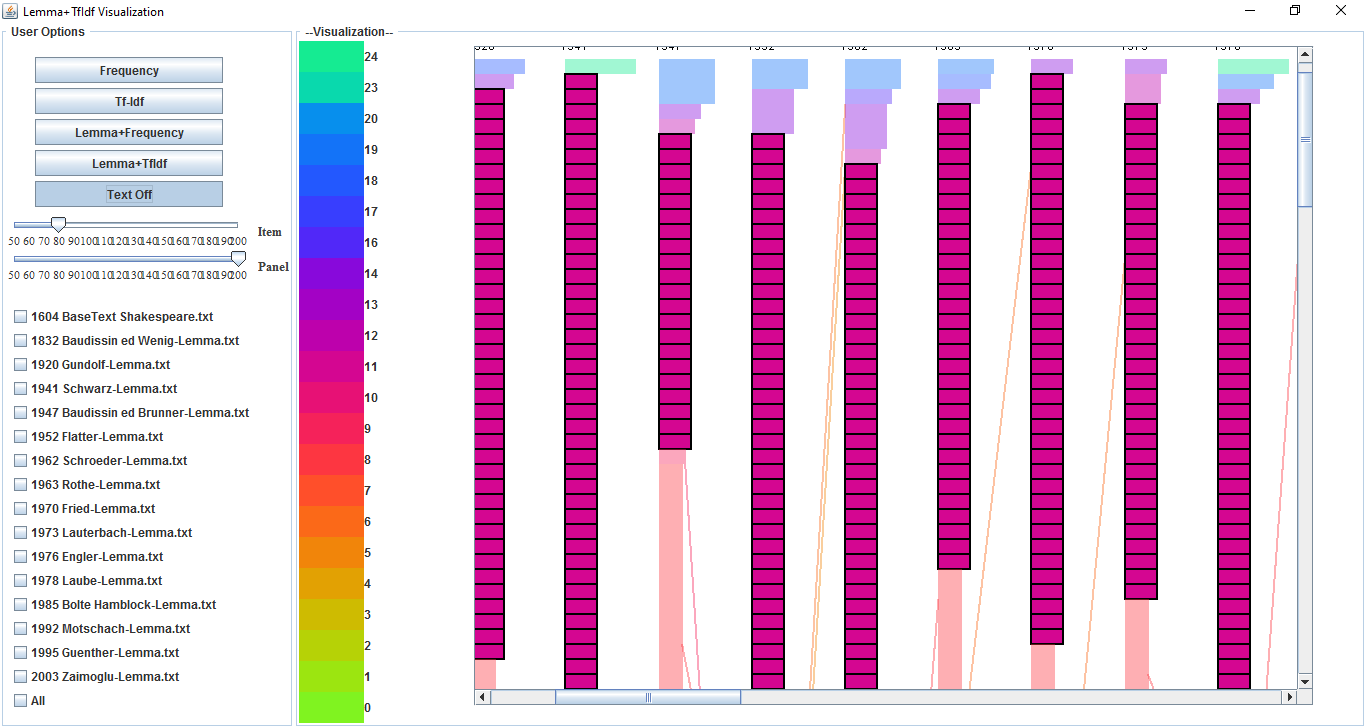
\includegraphics[width=16cm, height=12cm]{Figs/Colour-Legend-Interation}\\[1ex]
	\caption{}
	\label{fig:interactiveColourMapping}
\end{figure} 

\subsection{Lemmatisation}

The lemma visualisation a significant feature in this project. Lemma is a linguistic term which described as the dictionary form of a word. Take the English word 'decide' for example: 'decide' is the lemma for 'decided', 'decides', 'deciding'. Accordingly, lemmatisation is the process to obtain the lemma for each word. To achieve the effect of lemma view, several steps is necessary:
\begin{itemize}
	\item \textbf{} Obtain the German lemma corpus which contains an index of lemmas and words.
	\item \textbf{} Compare the words in our German translation corpus with the words in the German lemma corpus, and find the lemma for each term in our corpus.
	\item \textbf{} Store all the lemmas being found and generate a new lemma index.
	\item \textbf{} Apply the lemmas into visualisation.
\end{itemize}
For this project, an inevitable dilemma is the limited resources of German lemma corpus. As illustrated in Data Characteristics chapter, there is no relevant German lemma corpus in this project when we start this project. Also, German, as an affected language, is difficult to lemmatise. It is more challenging to acquire this kind of corpus from other sources. During this process, we attempted two solutions: Treetagger and DeReWo, which will be explained in following sections.

\subsubsection{TreeTagger}

As introduced in Technology Choices chapter, the TreeTagger is a tool for annotating text data and lemma information. Figure \ref{fig:treeTaggerUI} shows the Interface of TreeTagger. During applying this tool in the lemmatizing task of the project, we found this tool has following advantages:

\begin{figure}[h]
	\centering	
	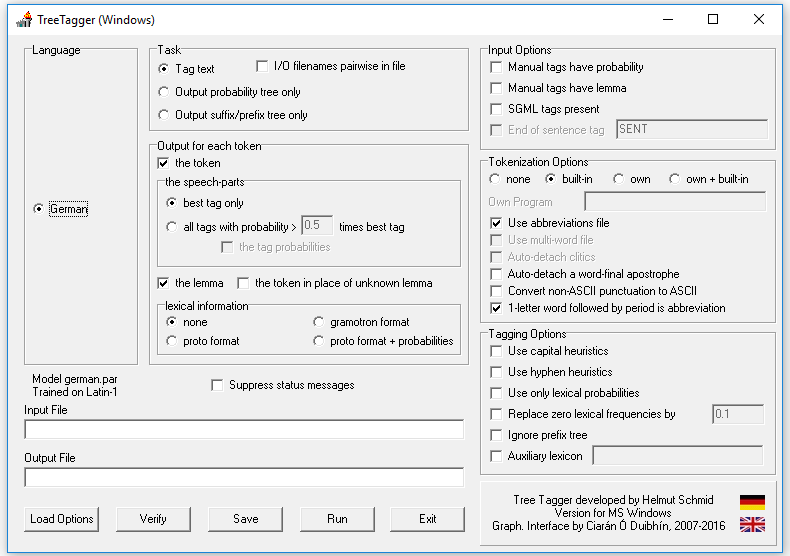
\includegraphics[width=16cm, height=12cm]{Figs/TreeTaggerInterface}\\[1ex]
	\caption{}
	\label{fig:treeTaggerUI}
\end{figure} 

\begin{itemize}
	\item \textbf{} The software is easy to obtain. Without any redundant procedures such as registration, the tool can be downloaded directly from the website \url{http://www.cis.uni-muenchen.de/~schmid/tools/TreeTagger/}.
	\item \textbf{} The user interface of the tool is clear and easy to use.
	\item \textbf{} The concept in using software is to upload a .txt file, create a .txt file to store results, and lemmatise the data.	
\end{itemize}

However, there are also some problems we encountered:
\begin{itemize}
	\item \textbf{} The format of the text file must be encoded in Latin-1, while the text file we have is encoded in UTF-8. Therefore, some German terms with special characters cannot be recognised by the tool.
	\item \textbf{} From the results we achieved, the tool cannot recognise words with capital letters. 
	\item \textbf{} The tool cannot be used to lemmatise a group of files at one time, which is not appropriate for project which needs to process large data sets. 	
\end{itemize}

We connected an domain expert, Dr. Tom Cheesman form the Mordern Language Center of Swansea University, to evaluate the results of the lemmatisation for TreeTagger. Appendix {?} is the file of sample lemma we sent to Dr. Cheesman with the comments he sent back. Due to the low accuracy of the results for the data in this project, this solution is given up in the end.

\subsubsection{DeReWo}

DeReWo is a project done by Institut Fur Deutsche Sprache. This project aims at developing methods to create frequncy-based ranking lists of lemma based on random virtual corpora. In the DeReWo website \url{http://www1.ids-mannheim.de/direktion/kl/projekte/methoden/derewo.html?L=1}, there are some downloadable resources of German lemma, including 'DeReKo-2014-II-MainArchive-STT.100000.freq', which is a file storing top 100,000 German words, lemmas and POS. The format of this document is .freq, which can be edit in Visual Studio Code. It also can be read from Java directly. Using this corpus, we successrully obtain all the lemmas for each term in the \emph{Othello} corpus for this project.

There are several phases of using DeReWo to generate lemma visualisation:
\begin{itemize}
	\item \textbf{} Read text file from \emph{Othello} corpus.	
	\item \textbf{} Read German lemma corpus file.
	\item \textbf{} Search for the lemma of each term.
	\item \textbf{} Store the lemma in a new text file. In this step, we create 15 .txt files for all German translation. Meanwhile, order of the lemma is kept as the same with their original text. For each version of \emph{Othello} translation, the two files (\emph{Othello} source file and lemma file) are served as an index for words and lemmas.
	\item \textbf{} Replace all terms with according lemmas and visualise the new results.
\end{itemize}	

Figure \ref{fig:lemmaView} shows the outcome of the lemma visualisation. 

\begin{figure}[h]
	\centering	
	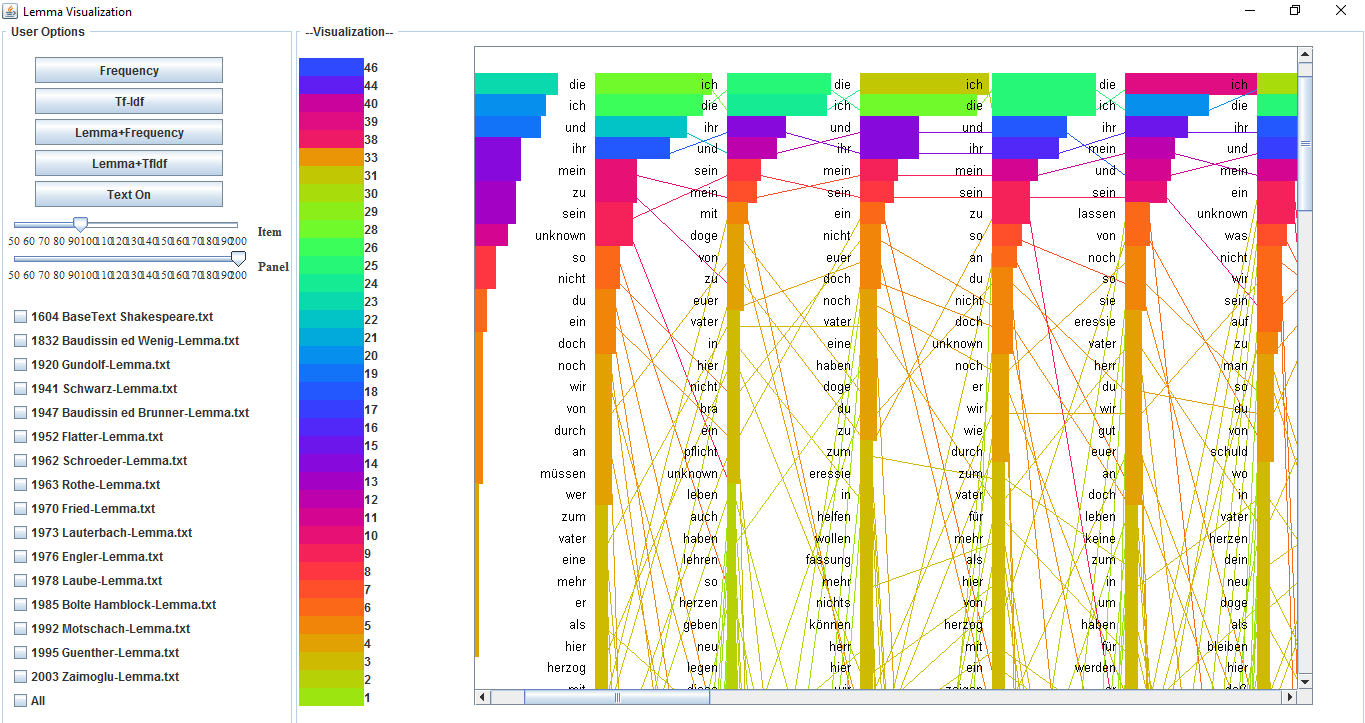
\includegraphics[width=16cm, height=12cm]{Figs/LemmaView}\\[1ex]
	\caption{}
	\label{fig:lemmaView}
\end{figure} 

\subsection{Tf-Idf}

Tf-Idf visualisation is an important feature in this project. As explained in Design chapter, the Tf-Idf value represents weightings of words, which also means we can get rid of unimportant words, namely stopping words. Therefore, the visualisation provided will be more helpful for researchers to study the varieties of translation. To fulfill this function, the most challenging step is to apply the formula of the Tf-Idf into the codes. Equation \ref{Tf-Idf} is used in this project to calculate the Tf-Idf value for each term \cite{Asking Mohammad about the equation referance}. The TfIdfCalculator class is created to process the Tf-Idf values.

The Tf-Idf visualisation generation process goes through the following steps:

\begin{itemize}
\item \textbf{} Calculate term frequency value. This step is done in the data reading stage. The Tf value hence can be achieved from DataReader object.
\item \textbf{} Calculate Idf value. As shown in Equation \ref{Tf-Idf},
\item \textbf{} Replace the frequency with Tf-Idf value.
\item \textbf{} Visulise according to new results.
\end{itemize} 

There are two visualisation generated using Tf-Idf value: one is to visualise data using Tf-Idf value and original words, as shown in Figure \ref{fig:tfIdfView}; the other is to visualise using Tf-Idf value together with lemma data which is displayed in Figure \ref{fig:tfIdfLemma}.

\begin{figure}[h]
	\centering	
	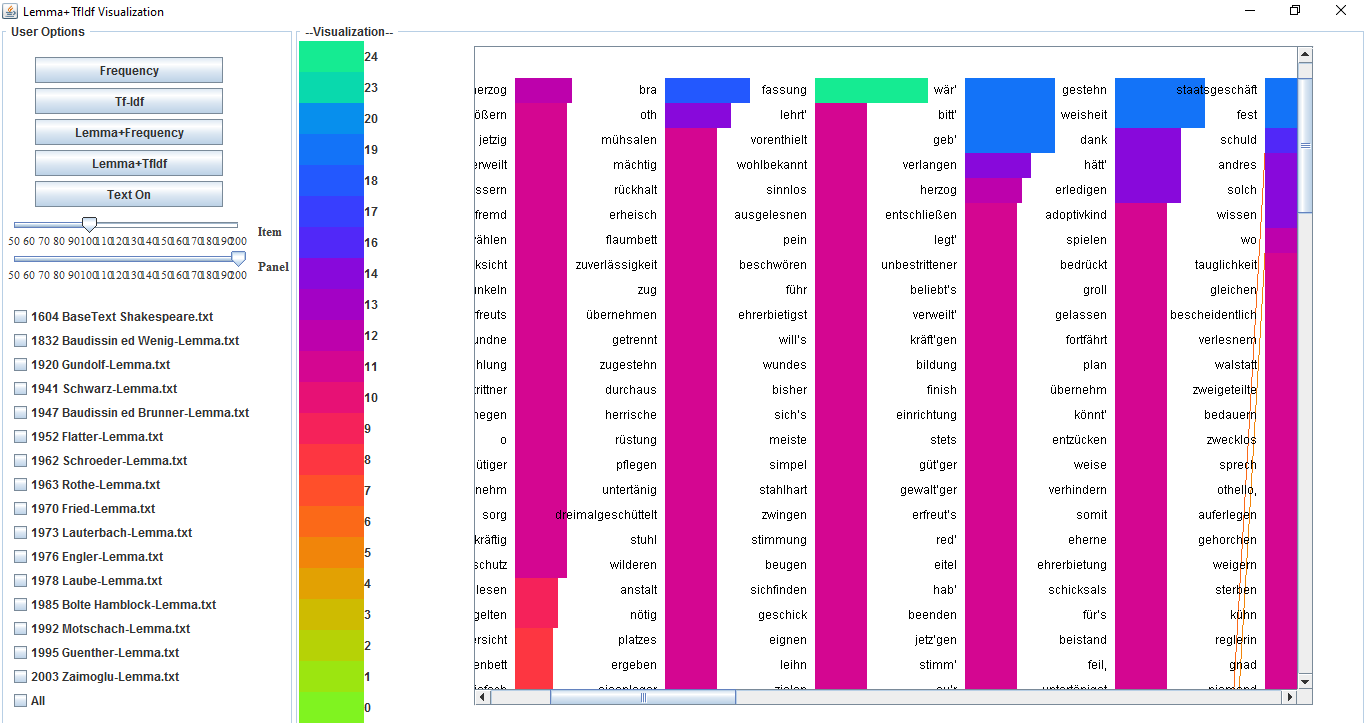
\includegraphics[width=16cm, height=12cm]{Figs/Lemma-Frequency}\\[1ex]
	\caption{}
	\label{fig:tfIdfView}
\end{figure} 
\begin{figure}[h]
	\centering	
	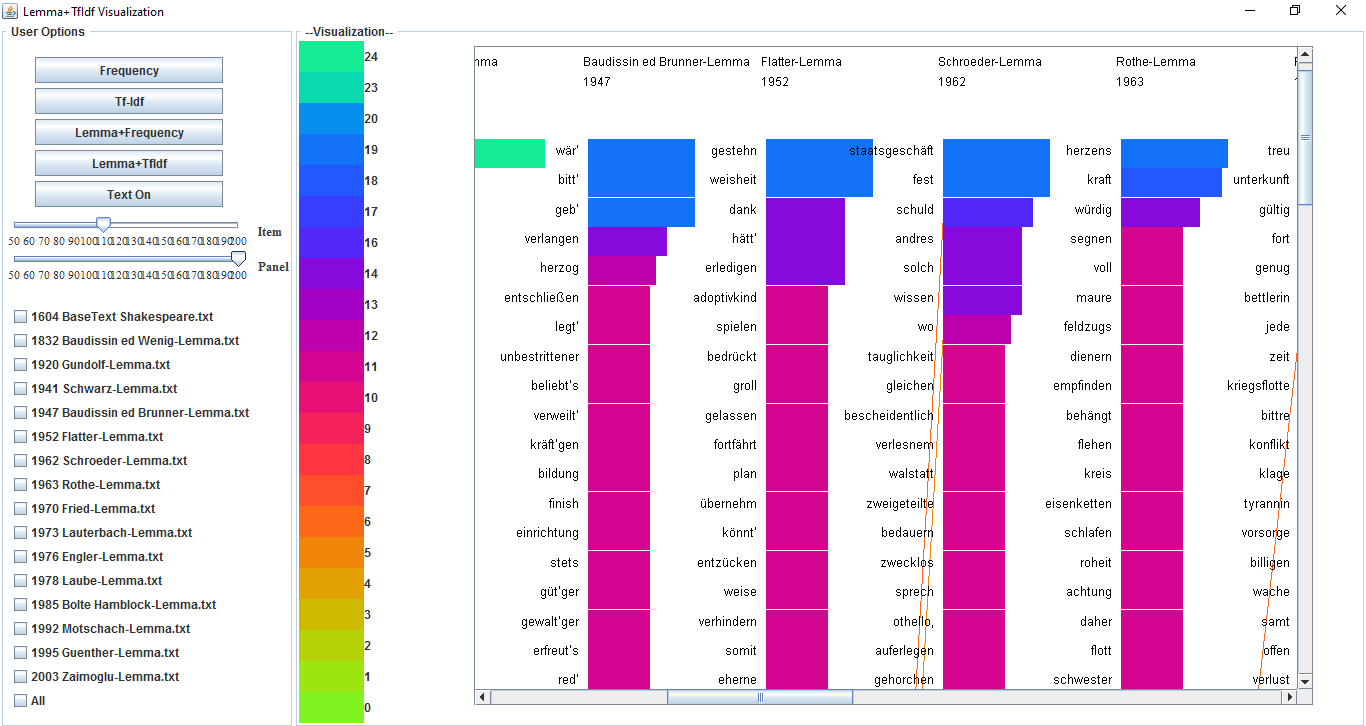
\includegraphics[width=16cm, height=12cm]{Figs/Lemma-TfIdf}\\[1ex]
	\caption{}
	\label{fig:tfIdfLemma}
\end{figure} 



%-----------------------------------------------------------------------------------------
\clearpage
\section{Evaluation}
%-----------------------------------------------------------------------------------------
In this section, we provide the description of the performance of the project, along with the illustration of our observations from the outcome of the visualizations. Feedback from a domain expert was also sought and forms part of this evaluation. evaluation.

\subsection{Results}

\paragraph{Frequency Visualisation}
\paragraph[]{}
The Frequency Visualisation is the basic feature and the primary task in this project. In this visualisation, we provided a parallel view of concordances to display the most frequent words in each version of the translation. As shown in \ref{fig:highlightView}, the colour of blocks differs from each other and the width of blocks represents ranges from the longest to the shortest. A highlight feature allows user to see same terms in each concordance.


However, from the results in the frequency visualisation, we can tell that the most frequent words in each version are the noise, and stop words such as 'ich' which means 'I' in English, or 'und' which means 'and' in English. These kinds of words are little help in translation comparison.


\paragraph{Tf-Idf Visualisation}
\paragraph[]{}The Tf-Idf Visualisation is another feature provided in this project. Based on features in Frequency Visualisation, the Tf-Idf Visualisation displays the most important words in the concordance. Therefore, the results of this visualisation are quite different compared to the Frequency Visualisation. In Figure \ref{fig:tfIdfView}, 27, terms in each concordance changed significantly. As illustrated in the Tf-Idf visualisation implementation section, if a word is listed on the top of a concordance, it means this word may appear many times in this version of the translation, while appearing not so frequently in the other concordance. For example, in Figure \ref{fig:fassung}, we see the word 'fassung' meaning 'composure' (in the 1941 version of the translation written by Schwarz) appears to have a high Tf-Idf value. When selecting 'fassung', it appears that no other blocks are highlighted, which means this word is not used by other authors. There are several guesses for this result:
\begin{itemize} 	
	\item \textbf{} The word 'fassung' is used multiple times in this translation version. So this is used to translate certain word or express specific meaning. (In this text, it is used to translate 'patience' or express 'the state of being calm and in control of oneself')
	\item \textbf{} This word does not appear in other versions, and we can assume that special trans- lation techniques were adopted, such as reformulation, adaptation, or compensation. 
	\item \textbf{} This unique outcome is likely because of  culture influences. Different cultural influences may lead to nuances in linguistic expression. In other words, the author may come from a distinct region when compared with other places and people can use different words to express the same meaning.
\end{itemize} 

\begin{figure}[H]
	\centering	
	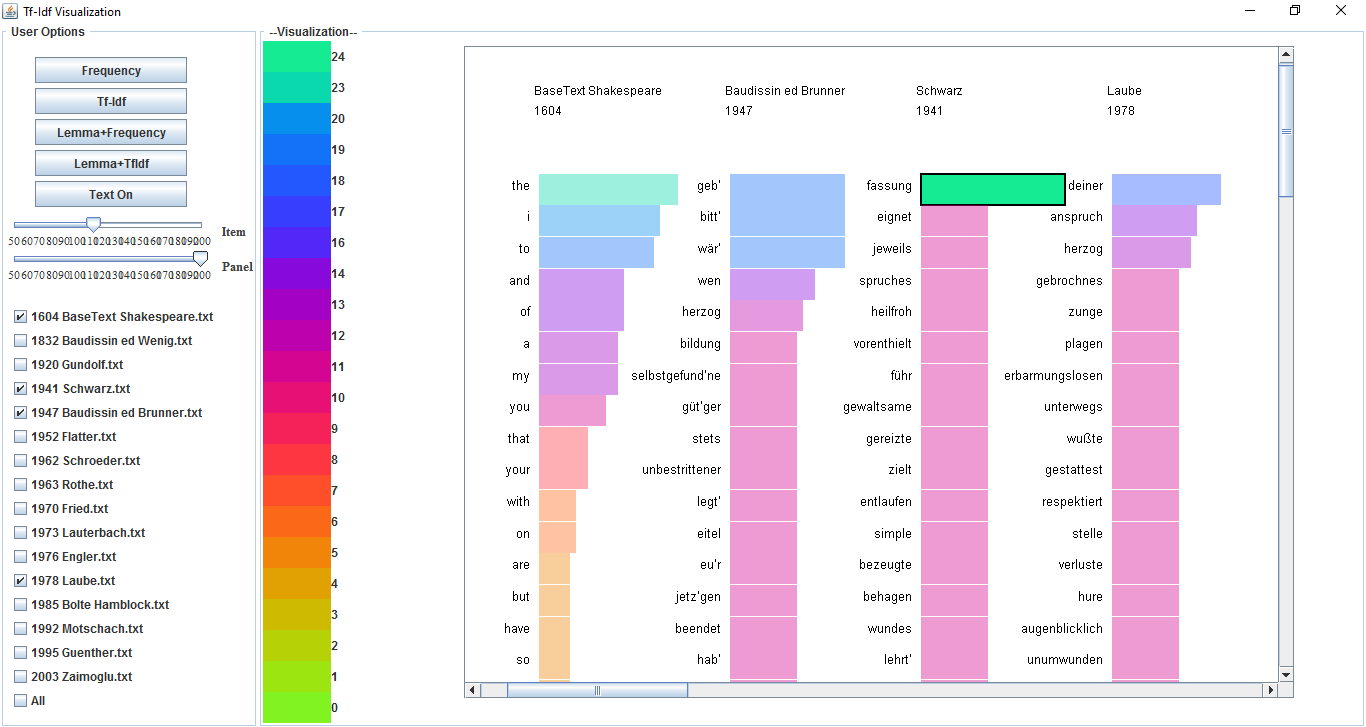
\includegraphics[scale=0.5]{Figs/Fassung}\\[1ex]
	\caption{The word 'fassung' is ranked high Tf-Idf value in one version}
	\label{fig:fassung}
\end{figure} 

\paragraph{Lemma Visualisation}
\paragraph[]{}Lemma Visualisation is generated after applying a lemma corpus to process our data. After lemmatisation, words are supposed to change into the original form, namely, the dictionary form (See Implementation chapter for relevant explanation). This feature is designed to combine the same words with different inflected forms. For example, the English word 'you' can be translated into 'dir', 'du', 'sie' and 'euch' in German. Figure \ref{fig:youInFreq} is the result after we select 'you' in the base text concordance. However, in Lemma Visualisation, only 'ihr' is highlighted.
 
\begin{figure}[H]
	\centering	
	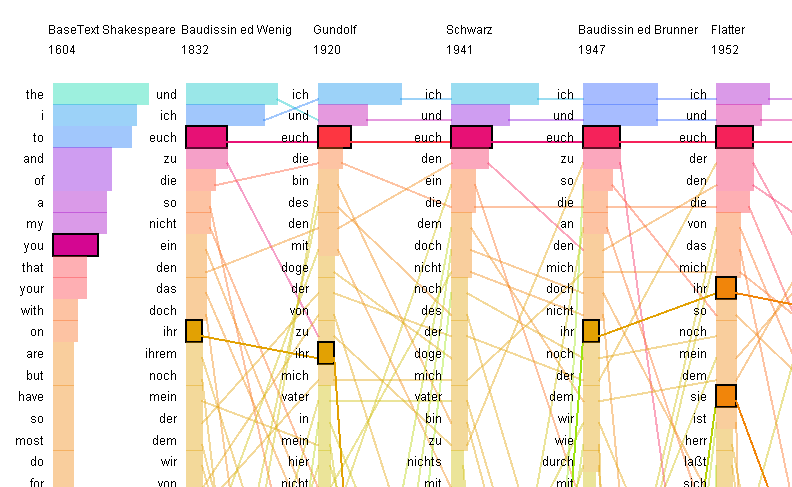
\includegraphics[scale=0.5]{Figs/You-In-Frequency}\\[1ex]
	\caption{ After clicking the block of English 'you' in base text, all German translations in other concordances are highlighted, such as  'dir', 'du', 'sie' , 'euch', and 'euch'.} 
	\label{fig:youInFreq}
\end{figure} 


\begin{figure}[H]
	\centering	
	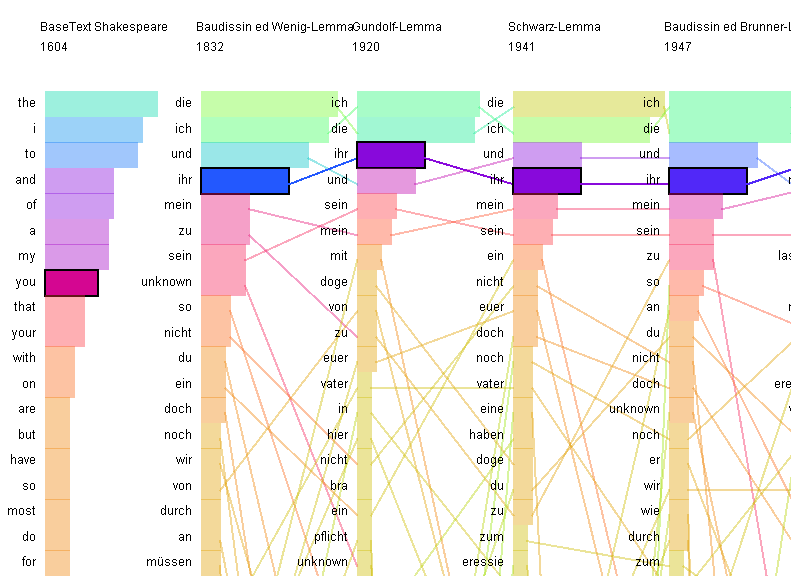
\includegraphics[scale=0.5]{Figs/You-In-Lemma}\\[1ex]
	\caption{After clicking the block of English 'you' in base text, only one German word is highlighted.}
	\label{fig:youInLemma}
\end{figure} 

As a result of lemmatisation, the length of column is shorter in the lemma view than in the frequency view. Also the frequency of words are changed. This can be seen from the colour legend in \ref{fig:freqLemmaComp}. Similarly it can be assumed that the variety of words are more obvious. However, more proofs and interpretations need to be explored in the future.

\begin{figure}[H]
	\centering	
	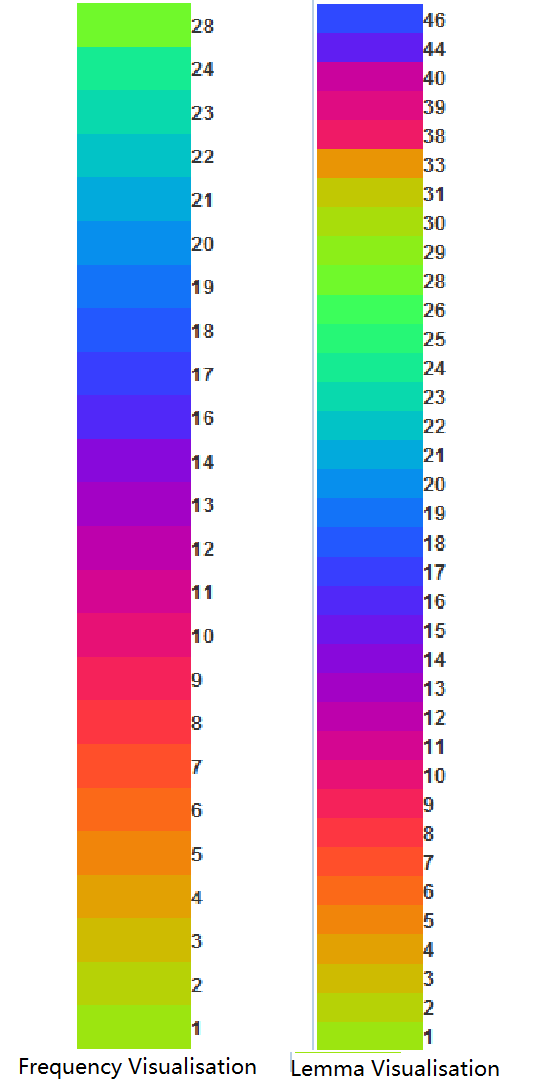
\includegraphics[scale=0.4]{Figs/Freq-Lemma-Comparison}\\[1ex]
	\caption{After combining the inflected form of words, the frequencies are incremented.} 
	\label{fig:freqLemmaComp}
\end{figure} 

\paragraph{Lemma and Tf-Idf Visualisation}
\paragraph[]{} The last view we rendered is the Lemma and Tf-Idf Visualisation. In this view, both the techniques of lemmatisation and Tf-Idf are utilized to display a parallel translation comparison in the software. From this visualisation, not only can we see the dictionary words, but the stop words are filtered. To prove the advantages of these results, two comparisons is necessary:
\begin{itemize} 	
	\item \textbf{Tf-Idf Visualisation vs Lemma and Tf-Idf Visualisation}\\
    The German word 'wen', meaning 'whom' in English, which bears little content information but merely performs grammar function. In Tf-Idf visualisation of Figure \ref{fig:tfIdfView}, the word 'wen' ranked on the top of second version from the left which is written by Baudissin ed Wenig in 1832 \cite{Hotho2005}. However, in Figure28, which applied both lemmatisation techiniques and Tf-Idf algorithm, this word disappears. This can be caused by the virtue that the word is combined with the dictionary word of 'wen', which has low Tf-Idf value.
	\item \textbf{Lemma Visualisation vs Lemma and Tf-Idf Visualisation}\\
If we only apply lemmatisation in the visualisation, stop words are still present. In Figure \ref{fig:lemmaView}, words such as 'die'('the' in English), 'ich'('I' in English), and 'und'('and' in English) are all considered as stop words \cite{Hotho2005}, which contribute little in translation studies. In the Lemma and Tf-Idf view, these words have disappeared because they are ranked to the bottom. 
\end{itemize}

\subsection{Domain Expert Feedback}

A domain expert, Dr. Tom Cheesman from the College of Art and Humanities at Swansea University, was invited as the user to give feedback on this project. During the meetings, we demonstrated the visualisations and features to him. The first one was organised on 13th November, 2017. Following the feedback, some features were overwritten and several new features were developed. The second meeting was on 4th December, 2017, in which he approved the new features.

\subsubsection{Session 1}

At this stage, Frequency Visualisation was finished, along with features such as turning the visualisation on and off, scaling the frame, version selection, and colour legend were implemented. Dr. Tom Cheesman expressed his interest by leaning his body to watch closer to 
the laptop. He asked some questions such as "What do the numbers beside colour legend represent?", "What are the connections?". He also requested that only the base text and three other German translations were shown so that he could understand the alignments. In the feed back, words like 'interesting', 'useful' and 'good' were used a lot. Meanwhile, other suggestions were mentioned and discussed, such as filtering stop words and seeing the most important words, together with showing the lemma of the words to decrease inflected words.

\subsubsection{Session 2}

In this stage, according to the feedback Dr. Cheesman gave at the first meeting, we did some more changes for the project: utilizing Tf-Idf algorithm in data processing, and using the German lemma corpus to lemmatize the terms. 

In the meeting, Dr. Cheesman expressed his interest and excitement by saying "This is good, this is pulling up some interesting stuff", "This is great...I can play with this". He showed great interest in the Lemma and Tf-Idf view, and pointed out some remarkable translations such as abbreviation words in the version written by Baudissin ed Brunner in 1947, (See Figure \ref{fig:feedback}). From the view, we can tell that more abbreviation words are used in this version which implies there is a unique translation strategy which the author uses. At the end of this meeting, Dr. Cheesman asked for a copy of the tools for assisting his translation studies.

\begin{figure}[H]
	\centering	
	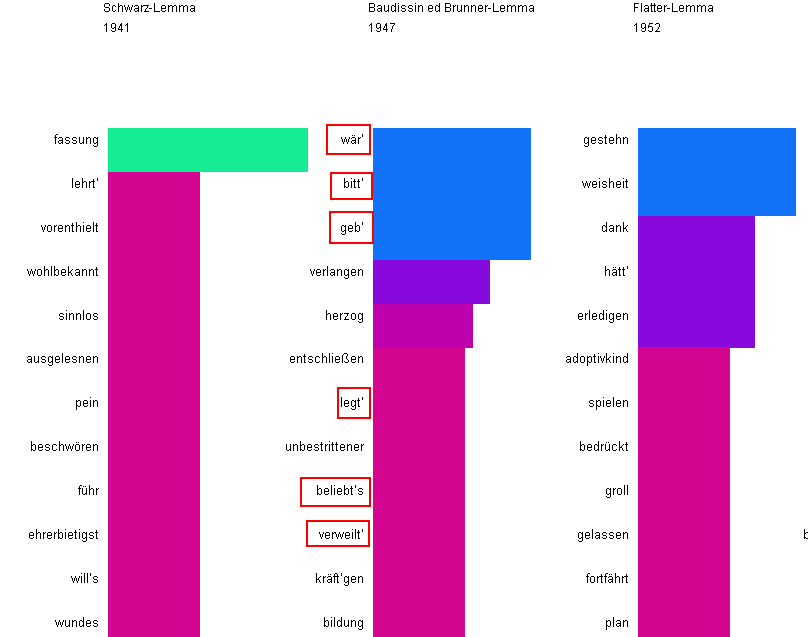
\includegraphics[scale=0.5]{Figs/Marking-Feedback}\\[1ex]
	\caption{After combining the inflected form of words, the frequencies are incremented.} 
	\label{fig:feedback}
\end{figure} 





%-----------------------------------------------------------------------------------------
\section{Future Work}
%-----------------------------------------------------------------------------------------

%-----------------------------------------------------------------------------------------
\section{Conclusion}
%-----------------------------------------------------------------------------------------
\lipsum[5-7]

%-----------------------------------------------------------------------------------------

\clearpage
\bibliographystyle{apalike}
\bibliography{References/TransVisReferences}

\clearpage
\begin{appendices}
\section{Minutes of Meeting }

\section{JavaDoc of Project }

pdf or latex

\end{appendices}
\end{document}
